\documentclass[twoside]{book}

% Packages required by doxygen
\usepackage{fixltx2e}
\usepackage{calc}
\usepackage{doxygen}
\usepackage{graphicx}
\usepackage[utf8]{inputenc}
\usepackage{makeidx}
\usepackage{multicol}
\usepackage{multirow}
\PassOptionsToPackage{warn}{textcomp}
\usepackage{textcomp}
\usepackage[nointegrals]{wasysym}
\usepackage[table]{xcolor}

% Font selection
\usepackage[T1]{fontenc}
\usepackage{mathptmx}
\usepackage[scaled=.90]{helvet}
\usepackage{courier}
\usepackage{amssymb}
\usepackage{sectsty}
\renewcommand{\familydefault}{\sfdefault}
\allsectionsfont{%
  \fontseries{bc}\selectfont%
  \color{darkgray}%
}
\renewcommand{\DoxyLabelFont}{%
  \fontseries{bc}\selectfont%
  \color{darkgray}%
}
\newcommand{\+}{\discretionary{\mbox{\scriptsize$\hookleftarrow$}}{}{}}

% Page & text layout
\usepackage{geometry}
\geometry{%
  a4paper,%
  top=2.5cm,%
  bottom=2.5cm,%
  left=2.5cm,%
  right=2.5cm%
}
\tolerance=750
\hfuzz=15pt
\hbadness=750
\setlength{\emergencystretch}{15pt}
\setlength{\parindent}{0cm}
\setlength{\parskip}{0.2cm}
\makeatletter
\renewcommand{\paragraph}{%
  \@startsection{paragraph}{4}{0ex}{-1.0ex}{1.0ex}{%
    \normalfont\normalsize\bfseries\SS@parafont%
  }%
}
\renewcommand{\subparagraph}{%
  \@startsection{subparagraph}{5}{0ex}{-1.0ex}{1.0ex}{%
    \normalfont\normalsize\bfseries\SS@subparafont%
  }%
}
\makeatother

% Headers & footers
\usepackage{fancyhdr}
\pagestyle{fancyplain}
\fancyhead[LE]{\fancyplain{}{\bfseries\thepage}}
\fancyhead[CE]{\fancyplain{}{}}
\fancyhead[RE]{\fancyplain{}{\bfseries\leftmark}}
\fancyhead[LO]{\fancyplain{}{\bfseries\rightmark}}
\fancyhead[CO]{\fancyplain{}{}}
\fancyhead[RO]{\fancyplain{}{\bfseries\thepage}}
\fancyfoot[LE]{\fancyplain{}{}}
\fancyfoot[CE]{\fancyplain{}{}}
\fancyfoot[RE]{\fancyplain{}{\bfseries\scriptsize Generated on Wed Mar 25 2015 16\+:13\+:15 for Projet\+\_\+\+R\+O by Doxygen }}
\fancyfoot[LO]{\fancyplain{}{\bfseries\scriptsize Generated on Wed Mar 25 2015 16\+:13\+:15 for Projet\+\_\+\+R\+O by Doxygen }}
\fancyfoot[CO]{\fancyplain{}{}}
\fancyfoot[RO]{\fancyplain{}{}}
\renewcommand{\footrulewidth}{0.4pt}
\renewcommand{\chaptermark}[1]{%
  \markboth{#1}{}%
}
\renewcommand{\sectionmark}[1]{%
  \markright{\thesection\ #1}%
}

% Indices & bibliography
\usepackage{natbib}
\usepackage[titles]{tocloft}
\setcounter{tocdepth}{3}
\setcounter{secnumdepth}{5}
\makeindex

% Hyperlinks (required, but should be loaded last)
\usepackage{ifpdf}
\ifpdf
  \usepackage[pdftex,pagebackref=true]{hyperref}
\else
  \usepackage[ps2pdf,pagebackref=true]{hyperref}
\fi
\hypersetup{%
  colorlinks=true,%
  linkcolor=blue,%
  citecolor=blue,%
  unicode%
}

% Custom commands
\newcommand{\clearemptydoublepage}{%
  \newpage{\pagestyle{empty}\cleardoublepage}%
}


%===== C O N T E N T S =====

\begin{document}

% Titlepage & ToC
\hypersetup{pageanchor=false,
             bookmarks=true,
             bookmarksnumbered=true,
             pdfencoding=unicode
            }
\pagenumbering{roman}
\begin{titlepage}
\vspace*{7cm}
\begin{center}%
{\Large Projet\+\_\+\+R\+O \\[1ex]\large v1.\+0 }\\
\vspace*{1cm}
{\large Generated by Doxygen 1.8.8}\\
\vspace*{0.5cm}
{\small Wed Mar 25 2015 16:13:15}\\
\end{center}
\end{titlepage}
\clearemptydoublepage
\tableofcontents
\clearemptydoublepage
\pagenumbering{arabic}
\hypersetup{pageanchor=true}

%--- Begin generated contents ---
\chapter{Hierarchical Index}
\section{Class Hierarchy}
This inheritance list is sorted roughly, but not completely, alphabetically\+:\begin{DoxyCompactList}
\item \contentsline{section}{Arete}{\pageref{class_arete}}{}
\item \contentsline{section}{Connexion}{\pageref{class_connexion}}{}
\item \contentsline{section}{Dessinable}{\pageref{class_dessinable}}{}
\begin{DoxyCompactList}
\item \contentsline{section}{Dessin\+Manager}{\pageref{class_dessin_manager}}{}
\end{DoxyCompactList}
\item \contentsline{section}{Etiquette}{\pageref{class_etiquette}}{}
\item exception\begin{DoxyCompactList}
\item \contentsline{section}{Exception}{\pageref{class_exception}}{}
\end{DoxyCompactList}
\item \contentsline{section}{Graphe}{\pageref{class_graphe}}{}
\item \contentsline{section}{Sommet}{\pageref{class_sommet}}{}
\item \contentsline{section}{Vecteur2\+D}{\pageref{class_vecteur2_d}}{}
\end{DoxyCompactList}

\chapter{Class Index}
\section{Class List}
Here are the classes, structs, unions and interfaces with brief descriptions\+:\begin{DoxyCompactList}
\item\contentsline{section}{\hyperlink{class_arete}{Arete} \\*The \hyperlink{class_arete}{Arete} class Cette classe sert à la représentation d'un \hyperlink{class_graphe}{Graphe}. Elle est définie par les deux sommets qu'elle relit, ansi qu'un coût et une ressource exprimé par des réels }{\pageref{class_arete}}{}
\item\contentsline{section}{\hyperlink{class_connexion}{Connexion} \\*The \hyperlink{class_connexion}{Connexion} class Cette classe est charg�e d'�tablire une connexion avec un serveur distant Cette classe charge une seule fois les dll Windows pour toutes les instances, cette partie est donc un singleton. De plus elle est compilable et fonctionnelle sous windows et unix(linux / mac compris) car la portabilit� c'est la vie }{\pageref{class_connexion}}{}
\item\contentsline{section}{\hyperlink{class_dessinable}{Dessinable} \\*The \hyperlink{class_dessinable}{Dessinable} class Il s'agit d'une interface décrivant le comportement que doivent avoir les classes de dessin. Cette classe sers donc majoritairement à assurer l'évolutivité de l'application en indiquant aux autres classes voulant dessiner les formes géometriques quelles méthodes elles doivent implémenter }{\pageref{class_dessinable}}{}
\item\contentsline{section}{\hyperlink{class_dessin_manager}{Dessin\+Manager} \\*The \hyperlink{class_dessin_manager}{Dessin\+Manager} class Cette classe est chargé de dessiner les formes géometriques. Le dessin est fait en envoyant les formes géometriques à un serveur distant afin que celui-\/ci dessine }{\pageref{class_dessin_manager}}{}
\item\contentsline{section}{\hyperlink{class_etiquette}{Etiquette} \\*The \hyperlink{class_etiquette}{Etiquette} class Cette classe représente une étiquette attachée à un sommet }{\pageref{class_etiquette}}{}
\item\contentsline{section}{\hyperlink{class_exception}{Exception} }{\pageref{class_exception}}{}
\item\contentsline{section}{\hyperlink{class_graphe}{Graphe} \\*The \hyperlink{class_graphe}{Graphe} class Cette classe représente un graphe. Elle est définie par une liste de sommets ainsi qu'une liste d'arêtes }{\pageref{class_graphe}}{}
\item\contentsline{section}{\hyperlink{class_sommet}{Sommet} \\*The \hyperlink{class_sommet}{Sommet} class Cette classe représente un sommet d'un graphe. Elle sert à la définition d'un graphe. Elle est composée d'un nom identifiant le sommet, ainsi qu'une fenêtre représenté par deux réels, et enfin par une liste d'étiquette rattachée au sommet }{\pageref{class_sommet}}{}
\item\contentsline{section}{\hyperlink{class_vecteur2_d}{Vecteur2\+D} }{\pageref{class_vecteur2_d}}{}
\end{DoxyCompactList}

\chapter{File Index}
\section{File List}
Here is a list of all files with brief descriptions\+:\begin{DoxyCompactList}
\item\contentsline{section}{\hyperlink{main_8cpp}{main.\+cpp} }{\pageref{main_8cpp}}{}
\item\contentsline{section}{Dessin/\hyperlink{connexion_8cpp}{connexion.\+cpp} }{\pageref{connexion_8cpp}}{}
\item\contentsline{section}{Dessin/\hyperlink{connexion_8h}{connexion.\+h} }{\pageref{connexion_8h}}{}
\item\contentsline{section}{Dessin/\hyperlink{dessinable_8h}{dessinable.\+h} }{\pageref{dessinable_8h}}{}
\item\contentsline{section}{Dessin/\hyperlink{dessin_manager_8cpp}{dessin\+Manager.\+cpp} }{\pageref{dessin_manager_8cpp}}{}
\item\contentsline{section}{Dessin/\hyperlink{dessin_manager_8h}{dessin\+Manager.\+h} }{\pageref{dessin_manager_8h}}{}
\item\contentsline{section}{Graphe/\hyperlink{_arete_8h}{Arete.\+h} }{\pageref{_arete_8h}}{}
\item\contentsline{section}{Graphe/\hyperlink{_etiquette_8h}{Etiquette.\+h} }{\pageref{_etiquette_8h}}{}
\item\contentsline{section}{Graphe/\hyperlink{_graphe_8h}{Graphe.\+h} }{\pageref{_graphe_8h}}{}
\item\contentsline{section}{Graphe/\hyperlink{_sommet_8h}{Sommet.\+h} }{\pageref{_sommet_8h}}{}
\item\contentsline{section}{Outils/\hyperlink{exception_8h}{exception.\+h} }{\pageref{exception_8h}}{}
\item\contentsline{section}{Outils/\hyperlink{tools_8h}{tools.\+h} }{\pageref{tools_8h}}{}
\item\contentsline{section}{Outils/\hyperlink{vecteur2d_8cpp}{vecteur2d.\+cpp} }{\pageref{vecteur2d_8cpp}}{}
\item\contentsline{section}{Outils/\hyperlink{vecteur2d_8h}{vecteur2d.\+h} }{\pageref{vecteur2d_8h}}{}
\end{DoxyCompactList}

\chapter{Class Documentation}
\hypertarget{class_arete}{\section{Arete Class Reference}
\label{class_arete}\index{Arete@{Arete}}
}


The \hyperlink{class_arete}{Arete} class Cette classe sert à la représentation d'un \hyperlink{class_graphe}{Graphe}. Elle est définie par les deux sommets qu'elle relit, ansi qu'un coût et une ressource exprimé par des réels.  




{\ttfamily \#include $<$Arete.\+h$>$}

\subsection*{Public Member Functions}
\begin{DoxyCompactItemize}
\item 
\hyperlink{class_arete_acdc3cd559c105c002ad10e66a2641ca9}{Arete} (\hyperlink{class_sommet}{Sommet} $\ast$\hyperlink{class_arete_abe2d1eac01195690e46bf61faab9493b}{from}, \hyperlink{class_sommet}{Sommet} $\ast$\hyperlink{class_arete_ae260ae83d6bbaaaf5547107fc40fec49}{to}, const double \&\hyperlink{class_arete_a082c784fbf985a8a991f3c035308fc0c}{cost}, const double \&\hyperlink{class_arete_a2f4d932778ea005c550473b39c5d7221}{resource})
\begin{DoxyCompactList}\small\item\em \hyperlink{class_arete}{Arete}. \end{DoxyCompactList}\item 
\hyperlink{class_arete_a27274ab782a462895e8218f41e957323}{operator string} () const 
\begin{DoxyCompactList}\small\item\em operator string \end{DoxyCompactList}\item 
\hyperlink{class_arete_ac557e81c9b02f266cadd55fd2952f377}{Arete} (\hyperlink{class_sommet}{Sommet} $\ast$\hyperlink{class_arete_abe2d1eac01195690e46bf61faab9493b}{from}, \hyperlink{class_sommet}{Sommet} $\ast$\hyperlink{class_arete_ae260ae83d6bbaaaf5547107fc40fec49}{to}, const double \&\hyperlink{class_arete_a082c784fbf985a8a991f3c035308fc0c}{cost})
\begin{DoxyCompactList}\small\item\em \hyperlink{class_arete}{Arete}. \end{DoxyCompactList}\item 
string \hyperlink{class_arete_af0a0e602373b28c3eb298ffd95c23aca}{to\+String} (bool rouge=true) const 
\begin{DoxyCompactList}\small\item\em to\+String \end{DoxyCompactList}\end{DoxyCompactItemize}
\subsection*{Public Attributes}
\begin{DoxyCompactItemize}
\item 
\hyperlink{class_sommet}{Sommet} $\ast$ \hyperlink{class_arete_abe2d1eac01195690e46bf61faab9493b}{from}
\item 
\hyperlink{class_sommet}{Sommet} $\ast$ \hyperlink{class_arete_ae260ae83d6bbaaaf5547107fc40fec49}{to}
\item 
double \hyperlink{class_arete_a082c784fbf985a8a991f3c035308fc0c}{cost}
\item 
double \hyperlink{class_arete_a2f4d932778ea005c550473b39c5d7221}{resource}
\end{DoxyCompactItemize}


\subsection{Detailed Description}
The \hyperlink{class_arete}{Arete} class Cette classe sert à la représentation d'un \hyperlink{class_graphe}{Graphe}. Elle est définie par les deux sommets qu'elle relit, ansi qu'un coût et une ressource exprimé par des réels. 

\subsection{Constructor \& Destructor Documentation}
\hypertarget{class_arete_acdc3cd559c105c002ad10e66a2641ca9}{\index{Arete@{Arete}!Arete@{Arete}}
\index{Arete@{Arete}!Arete@{Arete}}
\subsubsection[{Arete}]{\setlength{\rightskip}{0pt plus 5cm}Arete\+::\+Arete (
\begin{DoxyParamCaption}
\item[{{\bf Sommet} $\ast$}]{from, }
\item[{{\bf Sommet} $\ast$}]{to, }
\item[{const double \&}]{cost, }
\item[{const double \&}]{resource}
\end{DoxyParamCaption}
)\hspace{0.3cm}{\ttfamily [inline]}}}\label{class_arete_acdc3cd559c105c002ad10e66a2641ca9}


\hyperlink{class_arete}{Arete}. 


\begin{DoxyParams}{Parameters}
{\em from} & \hyperlink{class_sommet}{Sommet} de provenance \\
\hline
{\em to} & \hyperlink{class_sommet}{Sommet} de destination \\
\hline
{\em cost} & Coût de déplacement \\
\hline
{\em resource} & Ressource de déplacement \\
\hline
\end{DoxyParams}
\hypertarget{class_arete_ac557e81c9b02f266cadd55fd2952f377}{\index{Arete@{Arete}!Arete@{Arete}}
\index{Arete@{Arete}!Arete@{Arete}}
\subsubsection[{Arete}]{\setlength{\rightskip}{0pt plus 5cm}Arete\+::\+Arete (
\begin{DoxyParamCaption}
\item[{{\bf Sommet} $\ast$}]{from, }
\item[{{\bf Sommet} $\ast$}]{to, }
\item[{const double \&}]{cost}
\end{DoxyParamCaption}
)\hspace{0.3cm}{\ttfamily [inline]}}}\label{class_arete_ac557e81c9b02f266cadd55fd2952f377}


\hyperlink{class_arete}{Arete}. 


\begin{DoxyParams}{Parameters}
{\em from} & \hyperlink{class_sommet}{Sommet} de provenance \\
\hline
{\em to} & \hyperlink{class_sommet}{Sommet} de destination \\
\hline
{\em cost} & Coût de déplacement \\
\hline
\end{DoxyParams}


\subsection{Member Function Documentation}
\hypertarget{class_arete_a27274ab782a462895e8218f41e957323}{\index{Arete@{Arete}!operator string@{operator string}}
\index{operator string@{operator string}!Arete@{Arete}}
\subsubsection[{operator string}]{\setlength{\rightskip}{0pt plus 5cm}Arete\+::operator string (
\begin{DoxyParamCaption}
{}
\end{DoxyParamCaption}
) const\hspace{0.3cm}{\ttfamily [inline]}}}\label{class_arete_a27274ab782a462895e8218f41e957323}


operator string 

\hypertarget{class_arete_af0a0e602373b28c3eb298ffd95c23aca}{\index{Arete@{Arete}!to\+String@{to\+String}}
\index{to\+String@{to\+String}!Arete@{Arete}}
\subsubsection[{to\+String}]{\setlength{\rightskip}{0pt plus 5cm}string Arete\+::to\+String (
\begin{DoxyParamCaption}
\item[{bool}]{rouge = {\ttfamily true}}
\end{DoxyParamCaption}
) const\hspace{0.3cm}{\ttfamily [inline]}}}\label{class_arete_af0a0e602373b28c3eb298ffd95c23aca}


to\+String 


\begin{DoxyParams}{Parameters}
{\em rouge} & \\
\hline
\end{DoxyParams}
\begin{DoxyReturn}{Returns}

\end{DoxyReturn}


\subsection{Member Data Documentation}
\hypertarget{class_arete_a082c784fbf985a8a991f3c035308fc0c}{\index{Arete@{Arete}!cost@{cost}}
\index{cost@{cost}!Arete@{Arete}}
\subsubsection[{cost}]{\setlength{\rightskip}{0pt plus 5cm}double Arete\+::cost}}\label{class_arete_a082c784fbf985a8a991f3c035308fc0c}
\hypertarget{class_arete_abe2d1eac01195690e46bf61faab9493b}{\index{Arete@{Arete}!from@{from}}
\index{from@{from}!Arete@{Arete}}
\subsubsection[{from}]{\setlength{\rightskip}{0pt plus 5cm}{\bf Sommet}$\ast$ Arete\+::from}}\label{class_arete_abe2d1eac01195690e46bf61faab9493b}
\hypertarget{class_arete_a2f4d932778ea005c550473b39c5d7221}{\index{Arete@{Arete}!resource@{resource}}
\index{resource@{resource}!Arete@{Arete}}
\subsubsection[{resource}]{\setlength{\rightskip}{0pt plus 5cm}double Arete\+::resource}}\label{class_arete_a2f4d932778ea005c550473b39c5d7221}
\hypertarget{class_arete_ae260ae83d6bbaaaf5547107fc40fec49}{\index{Arete@{Arete}!to@{to}}
\index{to@{to}!Arete@{Arete}}
\subsubsection[{to}]{\setlength{\rightskip}{0pt plus 5cm}{\bf Sommet} $\ast$ Arete\+::to}}\label{class_arete_ae260ae83d6bbaaaf5547107fc40fec49}


The documentation for this class was generated from the following file\+:\begin{DoxyCompactItemize}
\item 
Graphe/\hyperlink{_arete_8h}{Arete.\+h}\end{DoxyCompactItemize}

\hypertarget{class_connexion}{\section{Connexion Class Reference}
\label{class_connexion}\index{Connexion@{Connexion}}
}


The \hyperlink{class_connexion}{Connexion} class Cette classe est charg�e d'�tablire une connexion avec un serveur distant Cette classe charge une seule fois les dll Windows pour toutes les instances, cette partie est donc un singleton. De plus elle est compilable et fonctionnelle sous windows et unix(linux / mac compris) car la portabilit� c'est la vie.  




{\ttfamily \#include $<$connexion.\+h$>$}

\subsection*{Public Member Functions}
\begin{DoxyCompactItemize}
\item 
\hyperlink{class_connexion_a7c890dbf77a2b9f49013a7be018d2230}{Connexion} (const std\+::string \&ip, int host)
\item 
void \hyperlink{class_connexion_aa8fbcb5c7ae95474159841a159075d72}{envoyer} (const char $\ast$) const 
\begin{DoxyCompactList}\small\item\em \hyperlink{class_connexion_aa8fbcb5c7ae95474159841a159075d72}{Connexion\+::envoyer} envoie le message au serveur. \end{DoxyCompactList}\item 
int \hyperlink{class_connexion_aff85c238e81fb5e3b7b5e218da2b70ef}{recevoir} () const 
\begin{DoxyCompactList}\small\item\em Dessin\+Manager\+::recevoir. \end{DoxyCompactList}\item 
\hyperlink{class_connexion_a6afee761c33e160c2be5e9e2713968e3}{$\sim$\+Connexion} ()
\end{DoxyCompactItemize}


\subsection{Detailed Description}
The \hyperlink{class_connexion}{Connexion} class Cette classe est charg�e d'�tablire une connexion avec un serveur distant Cette classe charge une seule fois les dll Windows pour toutes les instances, cette partie est donc un singleton. De plus elle est compilable et fonctionnelle sous windows et unix(linux / mac compris) car la portabilit� c'est la vie. 

\subsection{Constructor \& Destructor Documentation}
\hypertarget{class_connexion_a7c890dbf77a2b9f49013a7be018d2230}{\index{Connexion@{Connexion}!Connexion@{Connexion}}
\index{Connexion@{Connexion}!Connexion@{Connexion}}
\subsubsection[{Connexion}]{\setlength{\rightskip}{0pt plus 5cm}Connexion\+::\+Connexion (
\begin{DoxyParamCaption}
\item[{const std\+::string \&}]{ip, }
\item[{int}]{host}
\end{DoxyParamCaption}
)}}\label{class_connexion_a7c890dbf77a2b9f49013a7be018d2230}
\hypertarget{class_connexion_a6afee761c33e160c2be5e9e2713968e3}{\index{Connexion@{Connexion}!````~Connexion@{$\sim$\+Connexion}}
\index{````~Connexion@{$\sim$\+Connexion}!Connexion@{Connexion}}
\subsubsection[{$\sim$\+Connexion}]{\setlength{\rightskip}{0pt plus 5cm}Connexion\+::$\sim$\+Connexion (
\begin{DoxyParamCaption}
{}
\end{DoxyParamCaption}
)}}\label{class_connexion_a6afee761c33e160c2be5e9e2713968e3}


\subsection{Member Function Documentation}
\hypertarget{class_connexion_aa8fbcb5c7ae95474159841a159075d72}{\index{Connexion@{Connexion}!envoyer@{envoyer}}
\index{envoyer@{envoyer}!Connexion@{Connexion}}
\subsubsection[{envoyer}]{\setlength{\rightskip}{0pt plus 5cm}void Connexion\+::envoyer (
\begin{DoxyParamCaption}
\item[{const char $\ast$}]{message}
\end{DoxyParamCaption}
) const}}\label{class_connexion_aa8fbcb5c7ae95474159841a159075d72}


\hyperlink{class_connexion_aa8fbcb5c7ae95474159841a159075d72}{Connexion\+::envoyer} envoie le message au serveur. 


\begin{DoxyParams}{Parameters}
{\em message} & le message � envoyer Cette m�thode permet d'envoyer un message au serveur Il ne faut pas ajouter \char`\"{}\textbackslash{}r\textbackslash{}n\char`\"{} � la fin du message, la fonction s'en charge. \\
\hline
\end{DoxyParams}
\hypertarget{class_connexion_aff85c238e81fb5e3b7b5e218da2b70ef}{\index{Connexion@{Connexion}!recevoir@{recevoir}}
\index{recevoir@{recevoir}!Connexion@{Connexion}}
\subsubsection[{recevoir}]{\setlength{\rightskip}{0pt plus 5cm}int Connexion\+::recevoir (
\begin{DoxyParamCaption}
{}
\end{DoxyParamCaption}
) const}}\label{class_connexion_aff85c238e81fb5e3b7b5e218da2b70ef}


Dessin\+Manager\+::recevoir. 

\begin{DoxyReturn}{Returns}
la r�ponse du serveur, 0 (il y a eu une \hyperlink{class_exception}{Exception}) ou 1 (tout s'est bien pass�) Fonction � appeller apr�s chaque envoie de message, elle v�rifie que le message a bien �t� re�u par le serveur 
\end{DoxyReturn}


The documentation for this class was generated from the following files\+:\begin{DoxyCompactItemize}
\item 
Dessin/\hyperlink{connexion_8h}{connexion.\+h}\item 
Dessin/\hyperlink{connexion_8cpp}{connexion.\+cpp}\end{DoxyCompactItemize}

\hypertarget{class_dessinable}{\section{Dessinable Class Reference}
\label{class_dessinable}\index{Dessinable@{Dessinable}}
}


The \hyperlink{class_dessinable}{Dessinable} class Il s'agit d'une interface décrivant le comportement que doivent avoir les classes de dessin. Cette classe sers donc majoritairement à assurer l'évolutivité de l'application en indiquant aux autres classes voulant dessiner les formes géometriques quelles méthodes elles doivent implémenter.  




{\ttfamily \#include $<$dessinable.\+h$>$}

Inheritance diagram for Dessinable\+:\begin{figure}[H]
\begin{center}
\leavevmode
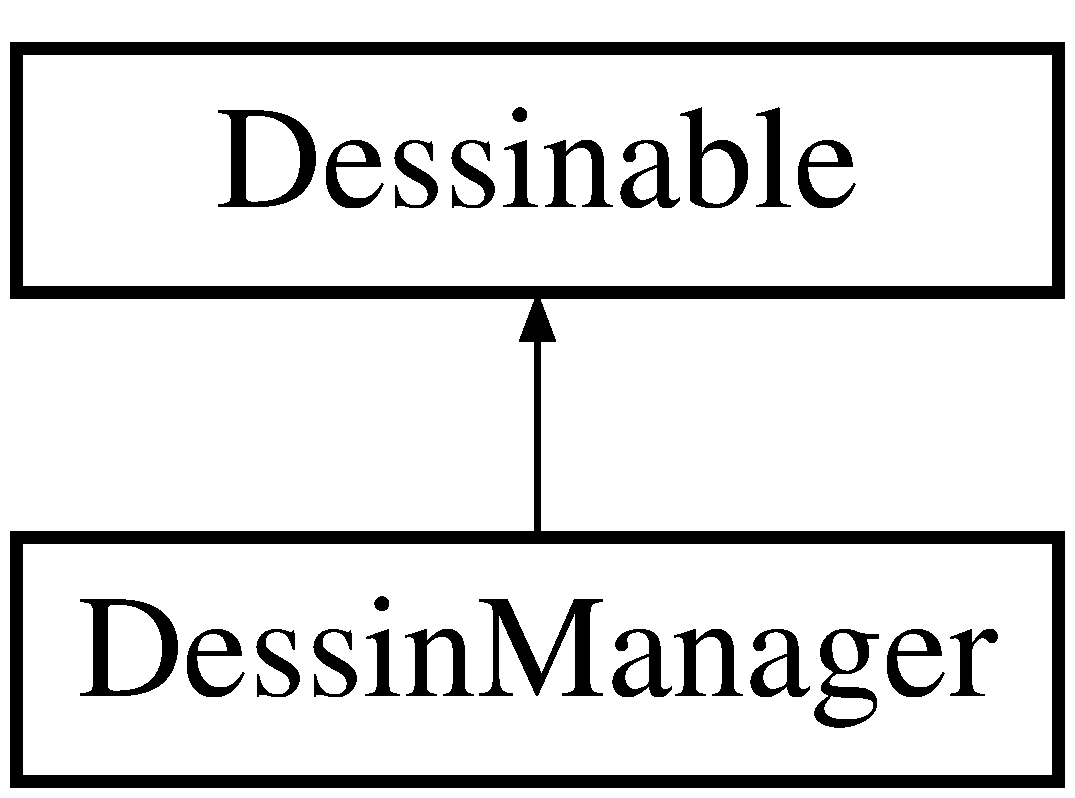
\includegraphics[height=2.000000cm]{class_dessinable}
\end{center}
\end{figure}
\subsection*{Public Member Functions}
\begin{DoxyCompactItemize}
\item 
virtual void \hyperlink{class_dessinable_a8e19f229f68063ba9a5164ef269d294d}{dessiner\+Aretes} (const vector$<$ \hyperlink{class_arete}{Arete} $>$ \&va, bool graphe=true) const =0
\item 
virtual \hyperlink{class_dessinable_a36e721321d1ba4324f446445793e7100}{$\sim$\+Dessinable} ()
\end{DoxyCompactItemize}


\subsection{Detailed Description}
The \hyperlink{class_dessinable}{Dessinable} class Il s'agit d'une interface décrivant le comportement que doivent avoir les classes de dessin. Cette classe sers donc majoritairement à assurer l'évolutivité de l'application en indiquant aux autres classes voulant dessiner les formes géometriques quelles méthodes elles doivent implémenter. 

\subsection{Constructor \& Destructor Documentation}
\hypertarget{class_dessinable_a36e721321d1ba4324f446445793e7100}{\index{Dessinable@{Dessinable}!````~Dessinable@{$\sim$\+Dessinable}}
\index{````~Dessinable@{$\sim$\+Dessinable}!Dessinable@{Dessinable}}
\subsubsection[{$\sim$\+Dessinable}]{\setlength{\rightskip}{0pt plus 5cm}virtual Dessinable\+::$\sim$\+Dessinable (
\begin{DoxyParamCaption}
{}
\end{DoxyParamCaption}
)\hspace{0.3cm}{\ttfamily [inline]}, {\ttfamily [virtual]}}}\label{class_dessinable_a36e721321d1ba4324f446445793e7100}


\subsection{Member Function Documentation}
\hypertarget{class_dessinable_a8e19f229f68063ba9a5164ef269d294d}{\index{Dessinable@{Dessinable}!dessiner\+Aretes@{dessiner\+Aretes}}
\index{dessiner\+Aretes@{dessiner\+Aretes}!Dessinable@{Dessinable}}
\subsubsection[{dessiner\+Aretes}]{\setlength{\rightskip}{0pt plus 5cm}virtual void Dessinable\+::dessiner\+Aretes (
\begin{DoxyParamCaption}
\item[{const vector$<$ {\bf Arete} $>$ \&}]{va, }
\item[{bool}]{graphe = {\ttfamily true}}
\end{DoxyParamCaption}
) const\hspace{0.3cm}{\ttfamily [pure virtual]}}}\label{class_dessinable_a8e19f229f68063ba9a5164ef269d294d}


Implemented in \hyperlink{class_dessin_manager_a1ff8d659f99a5e799f5d6e19c8be97dc}{Dessin\+Manager}.



The documentation for this class was generated from the following file\+:\begin{DoxyCompactItemize}
\item 
Dessin/\hyperlink{dessinable_8h}{dessinable.\+h}\end{DoxyCompactItemize}

\hypertarget{class_dessin_manager}{\section{Dessin\+Manager Class Reference}
\label{class_dessin_manager}\index{Dessin\+Manager@{Dessin\+Manager}}
}


The \hyperlink{class_dessin_manager}{Dessin\+Manager} class Cette classe est chargé de dessiner les formes géometriques. Le dessin est fait en envoyant les formes géometriques à un serveur distant afin que celui-\/ci dessine.  




{\ttfamily \#include $<$dessin\+Manager.\+h$>$}

Inheritance diagram for Dessin\+Manager\+:\begin{figure}[H]
\begin{center}
\leavevmode
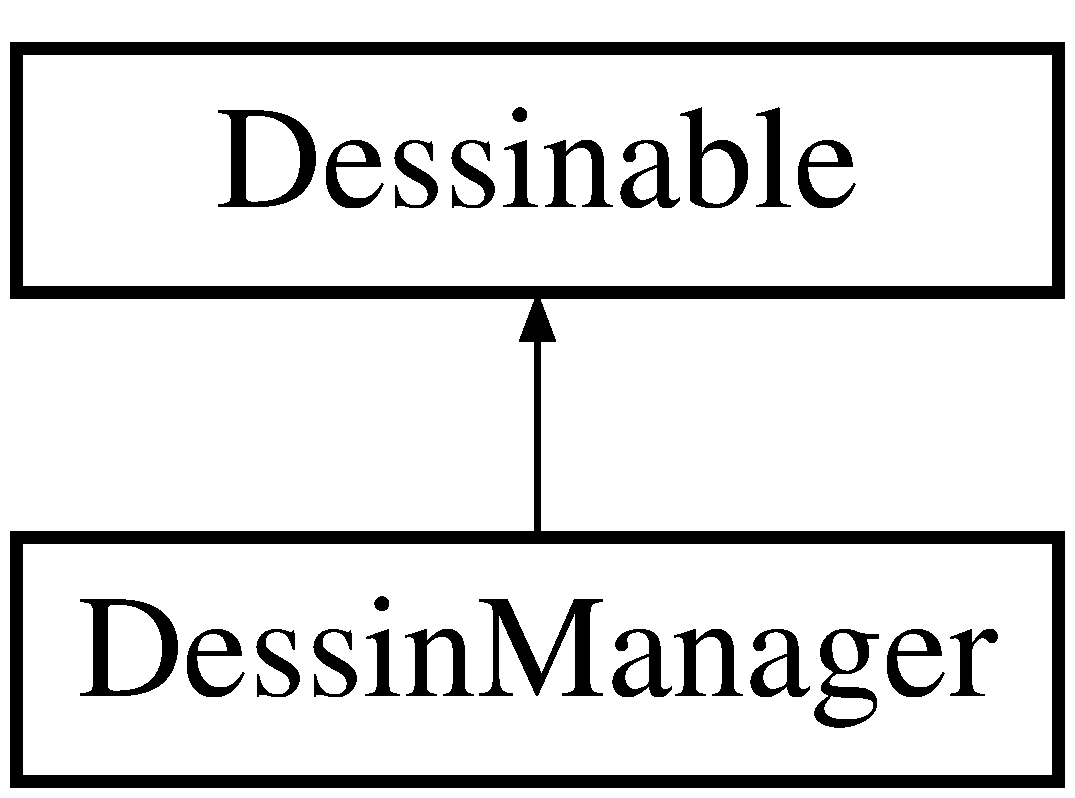
\includegraphics[height=2.000000cm]{class_dessin_manager}
\end{center}
\end{figure}
\subsection*{Public Member Functions}
\begin{DoxyCompactItemize}
\item 
\hyperlink{class_dessin_manager_ac3fc2fa6c1ac46893076b6b4529b8511}{Dessin\+Manager} (\hyperlink{class_connexion}{Connexion} $\ast$c)
\item 
virtual \hyperlink{class_dessin_manager_a1c10f7ad9be134e881db795c638883c5}{$\sim$\+Dessin\+Manager} ()
\item 
void \hyperlink{class_dessin_manager_a1ff8d659f99a5e799f5d6e19c8be97dc}{dessiner\+Aretes} (const vector$<$ \hyperlink{class_arete}{Arete} $>$ \&va, bool graphe) const 
\begin{DoxyCompactList}\small\item\em dessiner\+Aretes \end{DoxyCompactList}\item 
void \hyperlink{class_dessin_manager_a5f7b7feccd2c18af1d852c6ce78456c5}{dessiner\+Graphe} (const \hyperlink{class_graphe}{Graphe} \&G) const 
\end{DoxyCompactItemize}


\subsection{Detailed Description}
The \hyperlink{class_dessin_manager}{Dessin\+Manager} class Cette classe est chargé de dessiner les formes géometriques. Le dessin est fait en envoyant les formes géometriques à un serveur distant afin que celui-\/ci dessine. 

\subsection{Constructor \& Destructor Documentation}
\hypertarget{class_dessin_manager_ac3fc2fa6c1ac46893076b6b4529b8511}{\index{Dessin\+Manager@{Dessin\+Manager}!Dessin\+Manager@{Dessin\+Manager}}
\index{Dessin\+Manager@{Dessin\+Manager}!Dessin\+Manager@{Dessin\+Manager}}
\subsubsection[{Dessin\+Manager}]{\setlength{\rightskip}{0pt plus 5cm}Dessin\+Manager\+::\+Dessin\+Manager (
\begin{DoxyParamCaption}
\item[{{\bf Connexion} $\ast$}]{c}
\end{DoxyParamCaption}
)}}\label{class_dessin_manager_ac3fc2fa6c1ac46893076b6b4529b8511}
\hypertarget{class_dessin_manager_a1c10f7ad9be134e881db795c638883c5}{\index{Dessin\+Manager@{Dessin\+Manager}!````~Dessin\+Manager@{$\sim$\+Dessin\+Manager}}
\index{````~Dessin\+Manager@{$\sim$\+Dessin\+Manager}!Dessin\+Manager@{Dessin\+Manager}}
\subsubsection[{$\sim$\+Dessin\+Manager}]{\setlength{\rightskip}{0pt plus 5cm}virtual Dessin\+Manager\+::$\sim$\+Dessin\+Manager (
\begin{DoxyParamCaption}
{}
\end{DoxyParamCaption}
)\hspace{0.3cm}{\ttfamily [inline]}, {\ttfamily [virtual]}}}\label{class_dessin_manager_a1c10f7ad9be134e881db795c638883c5}


\subsection{Member Function Documentation}
\hypertarget{class_dessin_manager_a1ff8d659f99a5e799f5d6e19c8be97dc}{\index{Dessin\+Manager@{Dessin\+Manager}!dessiner\+Aretes@{dessiner\+Aretes}}
\index{dessiner\+Aretes@{dessiner\+Aretes}!Dessin\+Manager@{Dessin\+Manager}}
\subsubsection[{dessiner\+Aretes}]{\setlength{\rightskip}{0pt plus 5cm}void Dessin\+Manager\+::dessiner\+Aretes (
\begin{DoxyParamCaption}
\item[{const vector$<$ {\bf Arete} $>$ \&}]{va, }
\item[{bool}]{graphe = {\ttfamily true}}
\end{DoxyParamCaption}
) const\hspace{0.3cm}{\ttfamily [virtual]}}}\label{class_dessin_manager_a1ff8d659f99a5e799f5d6e19c8be97dc}


dessiner\+Aretes 


\begin{DoxyParams}{Parameters}
{\em va} & \\
\hline
{\em graphe} & true si on dessine un graphe, false si on dessine le chemin \\
\hline
\end{DoxyParams}


Implements \hyperlink{class_dessinable_a8e19f229f68063ba9a5164ef269d294d}{Dessinable}.

\hypertarget{class_dessin_manager_a5f7b7feccd2c18af1d852c6ce78456c5}{\index{Dessin\+Manager@{Dessin\+Manager}!dessiner\+Graphe@{dessiner\+Graphe}}
\index{dessiner\+Graphe@{dessiner\+Graphe}!Dessin\+Manager@{Dessin\+Manager}}
\subsubsection[{dessiner\+Graphe}]{\setlength{\rightskip}{0pt plus 5cm}void Dessin\+Manager\+::dessiner\+Graphe (
\begin{DoxyParamCaption}
\item[{const {\bf Graphe} \&}]{G}
\end{DoxyParamCaption}
) const}}\label{class_dessin_manager_a5f7b7feccd2c18af1d852c6ce78456c5}


The documentation for this class was generated from the following files\+:\begin{DoxyCompactItemize}
\item 
Dessin/\hyperlink{dessin_manager_8h}{dessin\+Manager.\+h}\item 
Dessin/\hyperlink{dessin_manager_8cpp}{dessin\+Manager.\+cpp}\end{DoxyCompactItemize}

\hypertarget{class_etiquette}{\section{Etiquette Class Reference}
\label{class_etiquette}\index{Etiquette@{Etiquette}}
}


The \hyperlink{class_etiquette}{Etiquette} class Cette classe représente une étiquette attachée à un sommet.  




{\ttfamily \#include $<$Etiquette.\+h$>$}

\subsection*{Public Member Functions}
\begin{DoxyCompactItemize}
\item 
\hyperlink{class_etiquette_a8b948d9bbaf895a2d66568f5e57c7de3}{Etiquette} (const \hyperlink{class_etiquette}{Etiquette} \&e)
\begin{DoxyCompactList}\small\item\em \hyperlink{class_etiquette}{Etiquette}. \end{DoxyCompactList}\item 
\hyperlink{class_etiquette_a83a1072b91450c15983e2e8aa02407c0}{Etiquette} (const \hyperlink{class_etiquette}{Etiquette} $\ast$\hyperlink{class_etiquette_a18f4af505c332fe206d08598f6471e46}{from}, const \hyperlink{class_sommet}{Sommet} $\ast$\hyperlink{class_etiquette_a8bd5882f6591338a62df5e5239103594}{to}, const double \&\hyperlink{class_etiquette_adb966761f009b397b8c70bcfed7f1c8c}{cost}, const double \&\hyperlink{class_etiquette_a12d2960b9e33da5ff3b0e1352bd1e4b2}{resources})
\begin{DoxyCompactList}\small\item\em \hyperlink{class_etiquette}{Etiquette}. \end{DoxyCompactList}\item 
\hyperlink{class_etiquette_a49a83a7682c03c2bf47b7f15cba8b479}{Etiquette} ()
\begin{DoxyCompactList}\small\item\em \hyperlink{class_etiquette}{Etiquette}. \end{DoxyCompactList}\item 
bool \hyperlink{class_etiquette_a3340880a27622cf152015cd731b9d131}{domine} (const \hyperlink{class_etiquette}{Etiquette} \&e)
\begin{DoxyCompactList}\small\item\em domine Vérifie si le cette étiquette domine celle passée en paramêtre. \end{DoxyCompactList}\item 
\hyperlink{class_etiquette_a77d0f0eeb7cc85094d3bb0153ececd44}{$\sim$\+Etiquette} ()
\item 
\hyperlink{class_etiquette_aa590c6f160a4e084559a7d286b01f4be}{operator string} () const 
\begin{DoxyCompactList}\small\item\em operator string \end{DoxyCompactList}\end{DoxyCompactItemize}
\subsection*{Public Attributes}
\begin{DoxyCompactItemize}
\item 
const \hyperlink{class_etiquette}{Etiquette} $\ast$ \hyperlink{class_etiquette_a18f4af505c332fe206d08598f6471e46}{from}
\item 
const \hyperlink{class_sommet}{Sommet} $\ast$ \hyperlink{class_etiquette_a8bd5882f6591338a62df5e5239103594}{to}
\item 
double \hyperlink{class_etiquette_adb966761f009b397b8c70bcfed7f1c8c}{cost}
\item 
double \hyperlink{class_etiquette_a12d2960b9e33da5ff3b0e1352bd1e4b2}{resources}
\end{DoxyCompactItemize}


\subsection{Detailed Description}
The \hyperlink{class_etiquette}{Etiquette} class Cette classe représente une étiquette attachée à un sommet. 

\subsection{Constructor \& Destructor Documentation}
\hypertarget{class_etiquette_a8b948d9bbaf895a2d66568f5e57c7de3}{\index{Etiquette@{Etiquette}!Etiquette@{Etiquette}}
\index{Etiquette@{Etiquette}!Etiquette@{Etiquette}}
\subsubsection[{Etiquette}]{\setlength{\rightskip}{0pt plus 5cm}Etiquette\+::\+Etiquette (
\begin{DoxyParamCaption}
\item[{const {\bf Etiquette} \&}]{e}
\end{DoxyParamCaption}
)\hspace{0.3cm}{\ttfamily [inline]}}}\label{class_etiquette_a8b948d9bbaf895a2d66568f5e57c7de3}


\hyperlink{class_etiquette}{Etiquette}. 


\begin{DoxyParams}{Parameters}
{\em e} & \\
\hline
\end{DoxyParams}
\hypertarget{class_etiquette_a83a1072b91450c15983e2e8aa02407c0}{\index{Etiquette@{Etiquette}!Etiquette@{Etiquette}}
\index{Etiquette@{Etiquette}!Etiquette@{Etiquette}}
\subsubsection[{Etiquette}]{\setlength{\rightskip}{0pt plus 5cm}Etiquette\+::\+Etiquette (
\begin{DoxyParamCaption}
\item[{const {\bf Etiquette} $\ast$}]{from, }
\item[{const {\bf Sommet} $\ast$}]{to, }
\item[{const double \&}]{cost, }
\item[{const double \&}]{resources}
\end{DoxyParamCaption}
)\hspace{0.3cm}{\ttfamily [inline]}}}\label{class_etiquette_a83a1072b91450c15983e2e8aa02407c0}


\hyperlink{class_etiquette}{Etiquette}. 


\begin{DoxyParams}{Parameters}
{\em from} & \\
\hline
{\em to} & \\
\hline
{\em cost} & \\
\hline
{\em resources} & \\
\hline
\end{DoxyParams}
\hypertarget{class_etiquette_a49a83a7682c03c2bf47b7f15cba8b479}{\index{Etiquette@{Etiquette}!Etiquette@{Etiquette}}
\index{Etiquette@{Etiquette}!Etiquette@{Etiquette}}
\subsubsection[{Etiquette}]{\setlength{\rightskip}{0pt plus 5cm}Etiquette\+::\+Etiquette (
\begin{DoxyParamCaption}
{}
\end{DoxyParamCaption}
)\hspace{0.3cm}{\ttfamily [inline]}}}\label{class_etiquette_a49a83a7682c03c2bf47b7f15cba8b479}


\hyperlink{class_etiquette}{Etiquette}. 

\hypertarget{class_etiquette_a77d0f0eeb7cc85094d3bb0153ececd44}{\index{Etiquette@{Etiquette}!````~Etiquette@{$\sim$\+Etiquette}}
\index{````~Etiquette@{$\sim$\+Etiquette}!Etiquette@{Etiquette}}
\subsubsection[{$\sim$\+Etiquette}]{\setlength{\rightskip}{0pt plus 5cm}Etiquette\+::$\sim$\+Etiquette (
\begin{DoxyParamCaption}
{}
\end{DoxyParamCaption}
)\hspace{0.3cm}{\ttfamily [inline]}}}\label{class_etiquette_a77d0f0eeb7cc85094d3bb0153ececd44}


\subsection{Member Function Documentation}
\hypertarget{class_etiquette_a3340880a27622cf152015cd731b9d131}{\index{Etiquette@{Etiquette}!domine@{domine}}
\index{domine@{domine}!Etiquette@{Etiquette}}
\subsubsection[{domine}]{\setlength{\rightskip}{0pt plus 5cm}bool Etiquette\+::domine (
\begin{DoxyParamCaption}
\item[{const {\bf Etiquette} \&}]{e}
\end{DoxyParamCaption}
)\hspace{0.3cm}{\ttfamily [inline]}}}\label{class_etiquette_a3340880a27622cf152015cd731b9d131}


domine Vérifie si le cette étiquette domine celle passée en paramêtre. 


\begin{DoxyParams}{Parameters}
{\em e} & \\
\hline
\end{DoxyParams}
\begin{DoxyReturn}{Returns}

\end{DoxyReturn}
\hypertarget{class_etiquette_aa590c6f160a4e084559a7d286b01f4be}{\index{Etiquette@{Etiquette}!operator string@{operator string}}
\index{operator string@{operator string}!Etiquette@{Etiquette}}
\subsubsection[{operator string}]{\setlength{\rightskip}{0pt plus 5cm}Etiquette\+::operator string (
\begin{DoxyParamCaption}
{}
\end{DoxyParamCaption}
) const\hspace{0.3cm}{\ttfamily [inline]}}}\label{class_etiquette_aa590c6f160a4e084559a7d286b01f4be}


operator string 



\subsection{Member Data Documentation}
\hypertarget{class_etiquette_adb966761f009b397b8c70bcfed7f1c8c}{\index{Etiquette@{Etiquette}!cost@{cost}}
\index{cost@{cost}!Etiquette@{Etiquette}}
\subsubsection[{cost}]{\setlength{\rightskip}{0pt plus 5cm}double Etiquette\+::cost}}\label{class_etiquette_adb966761f009b397b8c70bcfed7f1c8c}
\hypertarget{class_etiquette_a18f4af505c332fe206d08598f6471e46}{\index{Etiquette@{Etiquette}!from@{from}}
\index{from@{from}!Etiquette@{Etiquette}}
\subsubsection[{from}]{\setlength{\rightskip}{0pt plus 5cm}const {\bf Etiquette}$\ast$ Etiquette\+::from}}\label{class_etiquette_a18f4af505c332fe206d08598f6471e46}
\hypertarget{class_etiquette_a12d2960b9e33da5ff3b0e1352bd1e4b2}{\index{Etiquette@{Etiquette}!resources@{resources}}
\index{resources@{resources}!Etiquette@{Etiquette}}
\subsubsection[{resources}]{\setlength{\rightskip}{0pt plus 5cm}double Etiquette\+::resources}}\label{class_etiquette_a12d2960b9e33da5ff3b0e1352bd1e4b2}
\hypertarget{class_etiquette_a8bd5882f6591338a62df5e5239103594}{\index{Etiquette@{Etiquette}!to@{to}}
\index{to@{to}!Etiquette@{Etiquette}}
\subsubsection[{to}]{\setlength{\rightskip}{0pt plus 5cm}const {\bf Sommet}$\ast$ Etiquette\+::to}}\label{class_etiquette_a8bd5882f6591338a62df5e5239103594}


The documentation for this class was generated from the following file\+:\begin{DoxyCompactItemize}
\item 
Graphe/\hyperlink{_etiquette_8h}{Etiquette.\+h}\end{DoxyCompactItemize}

\hypertarget{class_exception}{\section{Exception Class Reference}
\label{class_exception}\index{Exception@{Exception}}
}


{\ttfamily \#include $<$exception.\+h$>$}

Inheritance diagram for Exception\+:\begin{figure}[H]
\begin{center}
\leavevmode
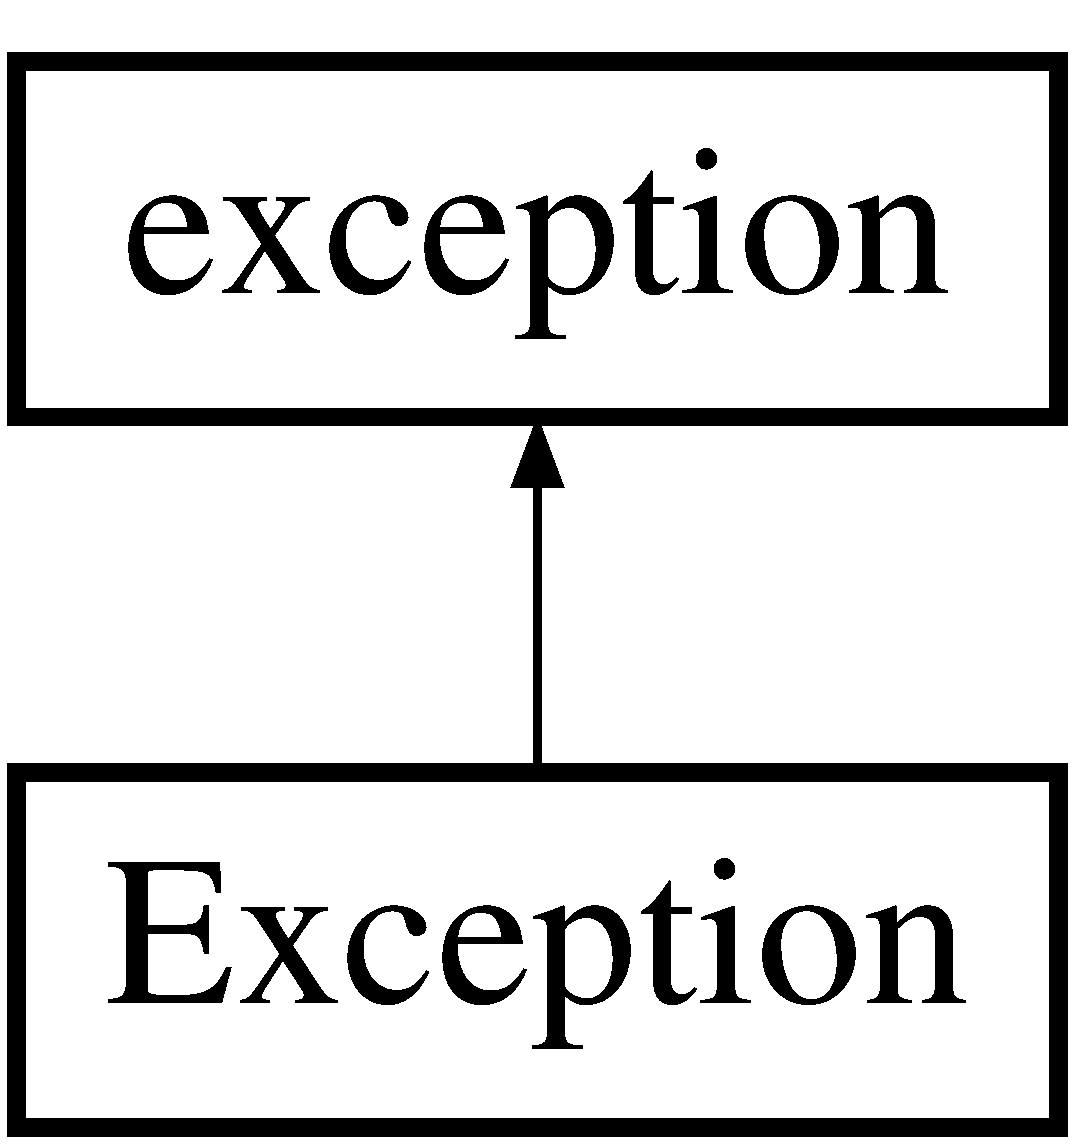
\includegraphics[height=2.000000cm]{class_exception}
\end{center}
\end{figure}
\subsection*{Public Member Functions}
\begin{DoxyCompactItemize}
\item 
\hyperlink{class_exception_a8f1884d73239c76f1a5ab4a4daa43ff1}{Exception} (std\+::string msg)
\item 
\hyperlink{class_exception_ad58328e3ace476630f34b47620e9846c}{Exception} (const char $\ast$c)
\item 
\hyperlink{class_exception_a60135107dc6351685a59a3e9b0aa005f}{Exception} (char $\ast$c)
\item 
virtual const char $\ast$ \hyperlink{class_exception_a78154a31544a609cbd226d32574f52cd}{what} () const   throw ()
\item 
virtual \hyperlink{class_exception_ad1ba411de295ef2eeb02ba26284a829a}{$\sim$\+Exception} ()  throw ()
\end{DoxyCompactItemize}
\subsection*{Public Attributes}
\begin{DoxyCompactItemize}
\item 
std\+::string \hyperlink{class_exception_a80bf622a8fc3c48fa6ab1a3fc024ff91}{message}
\end{DoxyCompactItemize}


\subsection{Constructor \& Destructor Documentation}
\hypertarget{class_exception_a8f1884d73239c76f1a5ab4a4daa43ff1}{\index{Exception@{Exception}!Exception@{Exception}}
\index{Exception@{Exception}!Exception@{Exception}}
\subsubsection[{Exception}]{\setlength{\rightskip}{0pt plus 5cm}Exception\+::\+Exception (
\begin{DoxyParamCaption}
\item[{std\+::string}]{msg}
\end{DoxyParamCaption}
)\hspace{0.3cm}{\ttfamily [inline]}}}\label{class_exception_a8f1884d73239c76f1a5ab4a4daa43ff1}
\hypertarget{class_exception_ad58328e3ace476630f34b47620e9846c}{\index{Exception@{Exception}!Exception@{Exception}}
\index{Exception@{Exception}!Exception@{Exception}}
\subsubsection[{Exception}]{\setlength{\rightskip}{0pt plus 5cm}Exception\+::\+Exception (
\begin{DoxyParamCaption}
\item[{const char $\ast$}]{c}
\end{DoxyParamCaption}
)\hspace{0.3cm}{\ttfamily [inline]}}}\label{class_exception_ad58328e3ace476630f34b47620e9846c}
\hypertarget{class_exception_a60135107dc6351685a59a3e9b0aa005f}{\index{Exception@{Exception}!Exception@{Exception}}
\index{Exception@{Exception}!Exception@{Exception}}
\subsubsection[{Exception}]{\setlength{\rightskip}{0pt plus 5cm}Exception\+::\+Exception (
\begin{DoxyParamCaption}
\item[{char $\ast$}]{c}
\end{DoxyParamCaption}
)\hspace{0.3cm}{\ttfamily [inline]}}}\label{class_exception_a60135107dc6351685a59a3e9b0aa005f}
\hypertarget{class_exception_ad1ba411de295ef2eeb02ba26284a829a}{\index{Exception@{Exception}!````~Exception@{$\sim$\+Exception}}
\index{````~Exception@{$\sim$\+Exception}!Exception@{Exception}}
\subsubsection[{$\sim$\+Exception}]{\setlength{\rightskip}{0pt plus 5cm}virtual Exception\+::$\sim$\+Exception (
\begin{DoxyParamCaption}
{}
\end{DoxyParamCaption}
) throw  ) \hspace{0.3cm}{\ttfamily [inline]}, {\ttfamily [virtual]}}}\label{class_exception_ad1ba411de295ef2eeb02ba26284a829a}


\subsection{Member Function Documentation}
\hypertarget{class_exception_a78154a31544a609cbd226d32574f52cd}{\index{Exception@{Exception}!what@{what}}
\index{what@{what}!Exception@{Exception}}
\subsubsection[{what}]{\setlength{\rightskip}{0pt plus 5cm}virtual const char$\ast$ Exception\+::what (
\begin{DoxyParamCaption}
{}
\end{DoxyParamCaption}
) const throw  ) \hspace{0.3cm}{\ttfamily [inline]}, {\ttfamily [virtual]}}}\label{class_exception_a78154a31544a609cbd226d32574f52cd}


\subsection{Member Data Documentation}
\hypertarget{class_exception_a80bf622a8fc3c48fa6ab1a3fc024ff91}{\index{Exception@{Exception}!message@{message}}
\index{message@{message}!Exception@{Exception}}
\subsubsection[{message}]{\setlength{\rightskip}{0pt plus 5cm}std\+::string Exception\+::message}}\label{class_exception_a80bf622a8fc3c48fa6ab1a3fc024ff91}


The documentation for this class was generated from the following file\+:\begin{DoxyCompactItemize}
\item 
Outils/\hyperlink{exception_8h}{exception.\+h}\end{DoxyCompactItemize}

\hypertarget{class_graphe}{\section{Graphe Class Reference}
\label{class_graphe}\index{Graphe@{Graphe}}
}


The \hyperlink{class_graphe}{Graphe} class Cette classe représente un graphe. Elle est définie par une liste de sommets ainsi qu'une liste d'arêtes.  




{\ttfamily \#include $<$Graphe.\+h$>$}

\subsection*{Public Member Functions}
\begin{DoxyCompactItemize}
\item 
\hyperlink{class_graphe_adb434f7fcd65a0da992946d699976808}{Graphe} (const string \&s)
\begin{DoxyCompactList}\small\item\em \hyperlink{class_graphe}{Graphe}. \end{DoxyCompactList}\item 
void \hyperlink{class_graphe_a99fc64177571ea73ae540fe27899e783}{add\+\_\+sommet} (const \hyperlink{class_sommet}{Sommet} \&s)
\begin{DoxyCompactList}\small\item\em add\+\_\+sommet Ajoute un sommet au graphe. \end{DoxyCompactList}\item 
void \hyperlink{class_graphe_aff29dc6bc5b4e5e028e12ac7e63571e6}{add\+\_\+successor} (\hyperlink{class_sommet}{Sommet} $\ast$from, \hyperlink{class_sommet}{Sommet} $\ast$to)
\begin{DoxyCompactList}\small\item\em add\+\_\+successor \end{DoxyCompactList}\item 
void \hyperlink{class_graphe_a4c845a9c2815cb68f3e9d075f40d5968}{add\+\_\+arete} (const \hyperlink{class_arete}{Arete} \&a)
\begin{DoxyCompactList}\small\item\em add\+\_\+arete Ajoute une arête au graphe \end{DoxyCompactList}\item 
void \hyperlink{class_graphe_a34df2e8f81e83ffde9feef6ac0bea29c}{add\+\_\+arete} (const string \&from, const string \&to, const double cost, const double resource)
\begin{DoxyCompactList}\small\item\em add\+\_\+arete Ajoute une arête au graphe \end{DoxyCompactList}\item 
virtual \hyperlink{class_graphe_a52fe805ae336c72b22b6d755822893b7}{$\sim$\+Graphe} ()
\begin{DoxyCompactList}\small\item\em $\sim$\+Graphe \end{DoxyCompactList}\item 
\hyperlink{class_sommet}{Sommet} $\ast$ \hyperlink{class_graphe_a78c033e49234a57fa86edbdcdc2c0da3}{find\+\_\+sommet} (const string \&\hyperlink{class_graphe_aba29a423311ef239951f6b6c37383444}{name})
\begin{DoxyCompactList}\small\item\em find\+\_\+sommet Recherche si le sommet identifié par son nom est contenu dans le graphe. \end{DoxyCompactList}\item 
\hyperlink{class_sommet}{Sommet} $\ast$ \hyperlink{class_graphe_af629041c83ff0754f0e1a7b3e9db5872}{find\+\_\+sommet} (const \hyperlink{class_sommet}{Sommet} \&s)
\begin{DoxyCompactList}\small\item\em find\+\_\+sommet \end{DoxyCompactList}\item 
\hyperlink{class_sommet}{Sommet} $\ast$ \hyperlink{class_graphe_a76b0a57584e44cbeef0a3563b6ec2751}{get\+\_\+sommet} (const string \&\hyperlink{class_graphe_aba29a423311ef239951f6b6c37383444}{name})
\begin{DoxyCompactList}\small\item\em get\+\_\+sommet \end{DoxyCompactList}\item 
vector$<$ \hyperlink{class_arete}{Arete} $>$ \hyperlink{class_graphe_ab9e88ea6bc8c5d7d4cd580e525e934b5}{correction\+\_\+etiquette} (const string \&from, const string \&to, \hyperlink{class_sommet}{Sommet} $\ast$\hyperlink{tools_8h_a677f6c8bffe4adb8d9d7359fdc40b142}{choisir}(const vector$<$ \hyperlink{class_sommet}{Sommet} $\ast$ $>$ \&list), vector$<$ \hyperlink{class_etiquette}{Etiquette} $\ast$ $>$ \hyperlink{tools_8h_a17cb87cf06a7862e3e44efe3ecdfb2fc}{pareto}(const vector$<$ \hyperlink{class_etiquette}{Etiquette} $\ast$ $>$ \&list))
\begin{DoxyCompactList}\small\item\em correction\+\_\+etiquette \end{DoxyCompactList}\item 
vector$<$ \hyperlink{class_arete}{Arete} $>$ \hyperlink{class_graphe_a334dcf698d519f22f276eda6d846a3de}{shortest\+\_\+path} (const \hyperlink{class_sommet}{Sommet} $\ast$from, const \hyperlink{class_sommet}{Sommet} $\ast$to)
\begin{DoxyCompactList}\small\item\em shortest\+\_\+path \end{DoxyCompactList}\item 
vector$<$ \hyperlink{class_arete}{Arete} $>$ \hyperlink{class_graphe_a39712d656bf8d7dbafbea4e0207565b3}{correction\+\_\+etiquette} (const \hyperlink{class_sommet}{Sommet} \&from, const \hyperlink{class_sommet}{Sommet} \&to, \hyperlink{class_sommet}{Sommet} $\ast$\hyperlink{tools_8h_a677f6c8bffe4adb8d9d7359fdc40b142}{choisir}(const vector$<$ \hyperlink{class_sommet}{Sommet} $\ast$ $>$ \&list), vector$<$ \hyperlink{class_etiquette}{Etiquette} $\ast$ $>$ \hyperlink{tools_8h_a17cb87cf06a7862e3e44efe3ecdfb2fc}{pareto}(const vector$<$ \hyperlink{class_etiquette}{Etiquette} $\ast$ $>$ \&list))
\begin{DoxyCompactList}\small\item\em correction\+\_\+etiquette \end{DoxyCompactList}\item 
\hyperlink{class_arete}{Arete} \hyperlink{class_graphe_a861e0c116f27493b176961bcb6daceee}{get\+\_\+arete} (const \hyperlink{class_sommet}{Sommet} $\ast$from, const \hyperlink{class_sommet}{Sommet} $\ast$to)
\begin{DoxyCompactList}\small\item\em get\+\_\+arete Retourne une arête identifiée par son sommet source et destination \end{DoxyCompactList}\item 
\hyperlink{class_arete}{Arete} \hyperlink{class_graphe_a048f84fc486a15cd69aad96fb93af08e}{get\+\_\+arete} (const string \&from, const string \&to)
\begin{DoxyCompactList}\small\item\em get\+\_\+arete Retourne une arête identifiée par le nom de son sommet source et destination \end{DoxyCompactList}\item 
\hyperlink{class_graphe_ac1174e4197d1a548bbaae047be13d61b}{operator string} () const 
\begin{DoxyCompactList}\small\item\em operator string \end{DoxyCompactList}\item 
const vector$<$ \hyperlink{class_arete}{Arete} $>$ \& \hyperlink{class_graphe_a43393cce73c8dba322682245585292e8}{get\+V\+Arete} () const 
\begin{DoxyCompactList}\small\item\em get\+V\+Arete \end{DoxyCompactList}\end{DoxyCompactItemize}
\subsection*{Static Public Member Functions}
\begin{DoxyCompactItemize}
\item 
static string \hyperlink{class_graphe_a9a646d290fb90eacf40c9747d2ef86b4}{format\+Du\+Prof} (const \hyperlink{class_graphe}{Graphe} \&G)
\begin{DoxyCompactList}\small\item\em format\+Du\+Prof \end{DoxyCompactList}\end{DoxyCompactItemize}
\subsection*{Public Attributes}
\begin{DoxyCompactItemize}
\item 
string \hyperlink{class_graphe_aba29a423311ef239951f6b6c37383444}{name}
\end{DoxyCompactItemize}


\subsection{Detailed Description}
The \hyperlink{class_graphe}{Graphe} class Cette classe représente un graphe. Elle est définie par une liste de sommets ainsi qu'une liste d'arêtes. 

\subsection{Constructor \& Destructor Documentation}
\hypertarget{class_graphe_adb434f7fcd65a0da992946d699976808}{\index{Graphe@{Graphe}!Graphe@{Graphe}}
\index{Graphe@{Graphe}!Graphe@{Graphe}}
\subsubsection[{Graphe}]{\setlength{\rightskip}{0pt plus 5cm}Graphe\+::\+Graphe (
\begin{DoxyParamCaption}
\item[{const string \&}]{s}
\end{DoxyParamCaption}
)\hspace{0.3cm}{\ttfamily [inline]}}}\label{class_graphe_adb434f7fcd65a0da992946d699976808}


\hyperlink{class_graphe}{Graphe}. 


\begin{DoxyParams}{Parameters}
{\em s} & \\
\hline
\end{DoxyParams}
\hypertarget{class_graphe_a52fe805ae336c72b22b6d755822893b7}{\index{Graphe@{Graphe}!````~Graphe@{$\sim$\+Graphe}}
\index{````~Graphe@{$\sim$\+Graphe}!Graphe@{Graphe}}
\subsubsection[{$\sim$\+Graphe}]{\setlength{\rightskip}{0pt plus 5cm}virtual Graphe\+::$\sim$\+Graphe (
\begin{DoxyParamCaption}
{}
\end{DoxyParamCaption}
)\hspace{0.3cm}{\ttfamily [inline]}, {\ttfamily [virtual]}}}\label{class_graphe_a52fe805ae336c72b22b6d755822893b7}


$\sim$\+Graphe 



\subsection{Member Function Documentation}
\hypertarget{class_graphe_a4c845a9c2815cb68f3e9d075f40d5968}{\index{Graphe@{Graphe}!add\+\_\+arete@{add\+\_\+arete}}
\index{add\+\_\+arete@{add\+\_\+arete}!Graphe@{Graphe}}
\subsubsection[{add\+\_\+arete}]{\setlength{\rightskip}{0pt plus 5cm}void Graphe\+::add\+\_\+arete (
\begin{DoxyParamCaption}
\item[{const {\bf Arete} \&}]{a}
\end{DoxyParamCaption}
)\hspace{0.3cm}{\ttfamily [inline]}}}\label{class_graphe_a4c845a9c2815cb68f3e9d075f40d5968}


add\+\_\+arete Ajoute une arête au graphe 


\begin{DoxyParams}{Parameters}
{\em a} & \\
\hline
\end{DoxyParams}
\hypertarget{class_graphe_a34df2e8f81e83ffde9feef6ac0bea29c}{\index{Graphe@{Graphe}!add\+\_\+arete@{add\+\_\+arete}}
\index{add\+\_\+arete@{add\+\_\+arete}!Graphe@{Graphe}}
\subsubsection[{add\+\_\+arete}]{\setlength{\rightskip}{0pt plus 5cm}void Graphe\+::add\+\_\+arete (
\begin{DoxyParamCaption}
\item[{const string \&}]{from, }
\item[{const string \&}]{to, }
\item[{const double}]{cost, }
\item[{const double}]{resource}
\end{DoxyParamCaption}
)\hspace{0.3cm}{\ttfamily [inline]}}}\label{class_graphe_a34df2e8f81e83ffde9feef6ac0bea29c}


add\+\_\+arete Ajoute une arête au graphe 


\begin{DoxyParams}{Parameters}
{\em from} & \\
\hline
{\em to} & \\
\hline
{\em cost} & \\
\hline
{\em resource} & \\
\hline
\end{DoxyParams}
\hypertarget{class_graphe_a99fc64177571ea73ae540fe27899e783}{\index{Graphe@{Graphe}!add\+\_\+sommet@{add\+\_\+sommet}}
\index{add\+\_\+sommet@{add\+\_\+sommet}!Graphe@{Graphe}}
\subsubsection[{add\+\_\+sommet}]{\setlength{\rightskip}{0pt plus 5cm}void Graphe\+::add\+\_\+sommet (
\begin{DoxyParamCaption}
\item[{const {\bf Sommet} \&}]{s}
\end{DoxyParamCaption}
)\hspace{0.3cm}{\ttfamily [inline]}}}\label{class_graphe_a99fc64177571ea73ae540fe27899e783}


add\+\_\+sommet Ajoute un sommet au graphe. 


\begin{DoxyParams}{Parameters}
{\em s} & \\
\hline
\end{DoxyParams}
\hypertarget{class_graphe_aff29dc6bc5b4e5e028e12ac7e63571e6}{\index{Graphe@{Graphe}!add\+\_\+successor@{add\+\_\+successor}}
\index{add\+\_\+successor@{add\+\_\+successor}!Graphe@{Graphe}}
\subsubsection[{add\+\_\+successor}]{\setlength{\rightskip}{0pt plus 5cm}void Graphe\+::add\+\_\+successor (
\begin{DoxyParamCaption}
\item[{{\bf Sommet} $\ast$}]{from, }
\item[{{\bf Sommet} $\ast$}]{to}
\end{DoxyParamCaption}
)\hspace{0.3cm}{\ttfamily [inline]}}}\label{class_graphe_aff29dc6bc5b4e5e028e12ac7e63571e6}


add\+\_\+successor 


\begin{DoxyParams}{Parameters}
{\em from} & \\
\hline
{\em to} & \\
\hline
\end{DoxyParams}
\hypertarget{class_graphe_ab9e88ea6bc8c5d7d4cd580e525e934b5}{\index{Graphe@{Graphe}!correction\+\_\+etiquette@{correction\+\_\+etiquette}}
\index{correction\+\_\+etiquette@{correction\+\_\+etiquette}!Graphe@{Graphe}}
\subsubsection[{correction\+\_\+etiquette}]{\setlength{\rightskip}{0pt plus 5cm}vector$<${\bf Arete}$>$ Graphe\+::correction\+\_\+etiquette (
\begin{DoxyParamCaption}
\item[{const string \&}]{from, }
\item[{const string \&}]{to, }
\item[{{\bf Sommet} $\ast$}]{choisirconst vector$<$ Sommet $\ast$ $>$ \&list, }
\item[{vector$<$ {\bf Etiquette} $\ast$ $>$ }]{paretoconst vector$<$ Etiquette $\ast$ $>$ \&list}
\end{DoxyParamCaption}
)\hspace{0.3cm}{\ttfamily [inline]}}}\label{class_graphe_ab9e88ea6bc8c5d7d4cd580e525e934b5}


correction\+\_\+etiquette 


\begin{DoxyParams}{Parameters}
{\em from} & \\
\hline
{\em to} & \\
\hline
{\em choisir} & \\
\hline
{\em pareto} & \\
\hline
\end{DoxyParams}
\begin{DoxyReturn}{Returns}

\end{DoxyReturn}
\hypertarget{class_graphe_a39712d656bf8d7dbafbea4e0207565b3}{\index{Graphe@{Graphe}!correction\+\_\+etiquette@{correction\+\_\+etiquette}}
\index{correction\+\_\+etiquette@{correction\+\_\+etiquette}!Graphe@{Graphe}}
\subsubsection[{correction\+\_\+etiquette}]{\setlength{\rightskip}{0pt plus 5cm}vector$<${\bf Arete}$>$ Graphe\+::correction\+\_\+etiquette (
\begin{DoxyParamCaption}
\item[{const {\bf Sommet} \&}]{from, }
\item[{const {\bf Sommet} \&}]{to, }
\item[{{\bf Sommet} $\ast$}]{choisirconst vector$<$ Sommet $\ast$ $>$ \&list, }
\item[{vector$<$ {\bf Etiquette} $\ast$ $>$ }]{paretoconst vector$<$ Etiquette $\ast$ $>$ \&list}
\end{DoxyParamCaption}
)\hspace{0.3cm}{\ttfamily [inline]}}}\label{class_graphe_a39712d656bf8d7dbafbea4e0207565b3}


correction\+\_\+etiquette 


\begin{DoxyParams}{Parameters}
{\em from} & \\
\hline
{\em to} & \\
\hline
{\em choisir} & \\
\hline
{\em pareto} & \\
\hline
\end{DoxyParams}
\begin{DoxyReturn}{Returns}

\end{DoxyReturn}
\hypertarget{class_graphe_a78c033e49234a57fa86edbdcdc2c0da3}{\index{Graphe@{Graphe}!find\+\_\+sommet@{find\+\_\+sommet}}
\index{find\+\_\+sommet@{find\+\_\+sommet}!Graphe@{Graphe}}
\subsubsection[{find\+\_\+sommet}]{\setlength{\rightskip}{0pt plus 5cm}{\bf Sommet}$\ast$ Graphe\+::find\+\_\+sommet (
\begin{DoxyParamCaption}
\item[{const string \&}]{name}
\end{DoxyParamCaption}
)\hspace{0.3cm}{\ttfamily [inline]}}}\label{class_graphe_a78c033e49234a57fa86edbdcdc2c0da3}


find\+\_\+sommet Recherche si le sommet identifié par son nom est contenu dans le graphe. 


\begin{DoxyParams}{Parameters}
{\em name} & \\
\hline
\end{DoxyParams}
\begin{DoxyReturn}{Returns}

\end{DoxyReturn}
\hypertarget{class_graphe_af629041c83ff0754f0e1a7b3e9db5872}{\index{Graphe@{Graphe}!find\+\_\+sommet@{find\+\_\+sommet}}
\index{find\+\_\+sommet@{find\+\_\+sommet}!Graphe@{Graphe}}
\subsubsection[{find\+\_\+sommet}]{\setlength{\rightskip}{0pt plus 5cm}{\bf Sommet}$\ast$ Graphe\+::find\+\_\+sommet (
\begin{DoxyParamCaption}
\item[{const {\bf Sommet} \&}]{s}
\end{DoxyParamCaption}
)\hspace{0.3cm}{\ttfamily [inline]}}}\label{class_graphe_af629041c83ff0754f0e1a7b3e9db5872}


find\+\_\+sommet 


\begin{DoxyParams}{Parameters}
{\em s} & \\
\hline
\end{DoxyParams}
\begin{DoxyReturn}{Returns}
le sommet dans le graphe ayant le même nom 
\end{DoxyReturn}
\hypertarget{class_graphe_a9a646d290fb90eacf40c9747d2ef86b4}{\index{Graphe@{Graphe}!format\+Du\+Prof@{format\+Du\+Prof}}
\index{format\+Du\+Prof@{format\+Du\+Prof}!Graphe@{Graphe}}
\subsubsection[{format\+Du\+Prof}]{\setlength{\rightskip}{0pt plus 5cm}static string Graphe\+::format\+Du\+Prof (
\begin{DoxyParamCaption}
\item[{const {\bf Graphe} \&}]{G}
\end{DoxyParamCaption}
)\hspace{0.3cm}{\ttfamily [inline]}, {\ttfamily [static]}}}\label{class_graphe_a9a646d290fb90eacf40c9747d2ef86b4}


format\+Du\+Prof 


\begin{DoxyParams}{Parameters}
{\em G} & \\
\hline
\end{DoxyParams}
\begin{DoxyReturn}{Returns}

\end{DoxyReturn}
\hypertarget{class_graphe_a861e0c116f27493b176961bcb6daceee}{\index{Graphe@{Graphe}!get\+\_\+arete@{get\+\_\+arete}}
\index{get\+\_\+arete@{get\+\_\+arete}!Graphe@{Graphe}}
\subsubsection[{get\+\_\+arete}]{\setlength{\rightskip}{0pt plus 5cm}{\bf Arete} Graphe\+::get\+\_\+arete (
\begin{DoxyParamCaption}
\item[{const {\bf Sommet} $\ast$}]{from, }
\item[{const {\bf Sommet} $\ast$}]{to}
\end{DoxyParamCaption}
)\hspace{0.3cm}{\ttfamily [inline]}}}\label{class_graphe_a861e0c116f27493b176961bcb6daceee}


get\+\_\+arete Retourne une arête identifiée par son sommet source et destination 


\begin{DoxyParams}{Parameters}
{\em from} & \\
\hline
{\em to} & \\
\hline
\end{DoxyParams}
\begin{DoxyReturn}{Returns}

\end{DoxyReturn}
\hypertarget{class_graphe_a048f84fc486a15cd69aad96fb93af08e}{\index{Graphe@{Graphe}!get\+\_\+arete@{get\+\_\+arete}}
\index{get\+\_\+arete@{get\+\_\+arete}!Graphe@{Graphe}}
\subsubsection[{get\+\_\+arete}]{\setlength{\rightskip}{0pt plus 5cm}{\bf Arete} Graphe\+::get\+\_\+arete (
\begin{DoxyParamCaption}
\item[{const string \&}]{from, }
\item[{const string \&}]{to}
\end{DoxyParamCaption}
)\hspace{0.3cm}{\ttfamily [inline]}}}\label{class_graphe_a048f84fc486a15cd69aad96fb93af08e}


get\+\_\+arete Retourne une arête identifiée par le nom de son sommet source et destination 


\begin{DoxyParams}{Parameters}
{\em from} & \\
\hline
{\em to} & \\
\hline
\end{DoxyParams}
\begin{DoxyReturn}{Returns}

\end{DoxyReturn}
\hypertarget{class_graphe_a76b0a57584e44cbeef0a3563b6ec2751}{\index{Graphe@{Graphe}!get\+\_\+sommet@{get\+\_\+sommet}}
\index{get\+\_\+sommet@{get\+\_\+sommet}!Graphe@{Graphe}}
\subsubsection[{get\+\_\+sommet}]{\setlength{\rightskip}{0pt plus 5cm}{\bf Sommet}$\ast$ Graphe\+::get\+\_\+sommet (
\begin{DoxyParamCaption}
\item[{const string \&}]{name}
\end{DoxyParamCaption}
)\hspace{0.3cm}{\ttfamily [inline]}}}\label{class_graphe_a76b0a57584e44cbeef0a3563b6ec2751}


get\+\_\+sommet 


\begin{DoxyParams}{Parameters}
{\em name} & \\
\hline
\end{DoxyParams}
\begin{DoxyReturn}{Returns}
le sommet dans le graphe ayant le même nom, s'il n'existe pas lève une exception 
\end{DoxyReturn}
\hypertarget{class_graphe_a43393cce73c8dba322682245585292e8}{\index{Graphe@{Graphe}!get\+V\+Arete@{get\+V\+Arete}}
\index{get\+V\+Arete@{get\+V\+Arete}!Graphe@{Graphe}}
\subsubsection[{get\+V\+Arete}]{\setlength{\rightskip}{0pt plus 5cm}const vector$<${\bf Arete}$>$\& Graphe\+::get\+V\+Arete (
\begin{DoxyParamCaption}
{}
\end{DoxyParamCaption}
) const\hspace{0.3cm}{\ttfamily [inline]}}}\label{class_graphe_a43393cce73c8dba322682245585292e8}


get\+V\+Arete 

\begin{DoxyReturn}{Returns}

\end{DoxyReturn}
\hypertarget{class_graphe_ac1174e4197d1a548bbaae047be13d61b}{\index{Graphe@{Graphe}!operator string@{operator string}}
\index{operator string@{operator string}!Graphe@{Graphe}}
\subsubsection[{operator string}]{\setlength{\rightskip}{0pt plus 5cm}Graphe\+::operator string (
\begin{DoxyParamCaption}
{}
\end{DoxyParamCaption}
) const\hspace{0.3cm}{\ttfamily [inline]}}}\label{class_graphe_ac1174e4197d1a548bbaae047be13d61b}


operator string 

\hypertarget{class_graphe_a334dcf698d519f22f276eda6d846a3de}{\index{Graphe@{Graphe}!shortest\+\_\+path@{shortest\+\_\+path}}
\index{shortest\+\_\+path@{shortest\+\_\+path}!Graphe@{Graphe}}
\subsubsection[{shortest\+\_\+path}]{\setlength{\rightskip}{0pt plus 5cm}vector$<${\bf Arete}$>$ Graphe\+::shortest\+\_\+path (
\begin{DoxyParamCaption}
\item[{const {\bf Sommet} $\ast$}]{from, }
\item[{const {\bf Sommet} $\ast$}]{to}
\end{DoxyParamCaption}
)\hspace{0.3cm}{\ttfamily [inline]}}}\label{class_graphe_a334dcf698d519f22f276eda6d846a3de}


shortest\+\_\+path 


\begin{DoxyParams}{Parameters}
{\em from} & \\
\hline
{\em to} & \\
\hline
\end{DoxyParams}
\begin{DoxyReturn}{Returns}

\end{DoxyReturn}


\subsection{Member Data Documentation}
\hypertarget{class_graphe_aba29a423311ef239951f6b6c37383444}{\index{Graphe@{Graphe}!name@{name}}
\index{name@{name}!Graphe@{Graphe}}
\subsubsection[{name}]{\setlength{\rightskip}{0pt plus 5cm}string Graphe\+::name}}\label{class_graphe_aba29a423311ef239951f6b6c37383444}


The documentation for this class was generated from the following file\+:\begin{DoxyCompactItemize}
\item 
Graphe/\hyperlink{_graphe_8h}{Graphe.\+h}\end{DoxyCompactItemize}

\hypertarget{class_sommet}{\section{Sommet Class Reference}
\label{class_sommet}\index{Sommet@{Sommet}}
}


The \hyperlink{class_sommet}{Sommet} class Cette classe représente un sommet d'un graphe. Elle sert à la définition d'un graphe. Elle est composée d'un nom identifiant le sommet, ainsi qu'une fenêtre représenté par deux réels, et enfin par une liste d'étiquette rattachée au sommet.  




{\ttfamily \#include $<$Sommet.\+h$>$}

\subsection*{Public Member Functions}
\begin{DoxyCompactItemize}
\item 
\hyperlink{class_sommet_a6a049f1ba2ad29a1e90d2b7825a94b02}{Sommet} ()
\begin{DoxyCompactList}\small\item\em \hyperlink{class_sommet}{Sommet}. \end{DoxyCompactList}\item 
\hyperlink{class_sommet_a2a63d8435ecad7a32deaeb9318ec0d9c}{Sommet} (const string \&\hyperlink{class_sommet_af32fce50ed4a5b4473722921986b34e5}{name})
\begin{DoxyCompactList}\small\item\em \hyperlink{class_sommet}{Sommet}. \end{DoxyCompactList}\item 
\hyperlink{class_sommet_a8ade745a2010341b78af423cfd64e114}{Sommet} (const string \&\hyperlink{class_sommet_af32fce50ed4a5b4473722921986b34e5}{name}, const double min, const double max)
\begin{DoxyCompactList}\small\item\em \hyperlink{class_sommet}{Sommet}. \end{DoxyCompactList}\item 
void \hyperlink{class_sommet_ae8446cb3c6230aa93cd519e7e8cd1fb5}{add\+\_\+tag} (const \hyperlink{class_etiquette}{Etiquette} \&e)
\begin{DoxyCompactList}\small\item\em add\+\_\+tag Ajoute une étiquette au sommet \end{DoxyCompactList}\item 
void \hyperlink{class_sommet_aba5faabbf46c0d14871c12a5002e990a}{add\+\_\+default\+\_\+tag} ()
\begin{DoxyCompactList}\small\item\em add\+\_\+default\+\_\+tag \end{DoxyCompactList}\item 
bool \hyperlink{class_sommet_a549e20bbfaafc40ad446c39919752edc}{operator==} (const \hyperlink{class_sommet}{Sommet} \&s) const 
\begin{DoxyCompactList}\small\item\em operator == \end{DoxyCompactList}\item 
\hyperlink{class_sommet_a73879831abd8a29cfed2d406fc0bcb3f}{operator string} () const 
\begin{DoxyCompactList}\small\item\em operator string \end{DoxyCompactList}\item 
virtual \hyperlink{class_sommet_a57d446e2ab9705b66fd869ac6ff5bee2}{$\sim$\+Sommet} ()
\begin{DoxyCompactList}\small\item\em $\sim$\+Sommet \end{DoxyCompactList}\item 
string \hyperlink{class_sommet_a7bc168163c08d358c69389df745a9115}{to\+String} () const 
\begin{DoxyCompactList}\small\item\em to\+String \end{DoxyCompactList}\end{DoxyCompactItemize}
\subsection*{Public Attributes}
\begin{DoxyCompactItemize}
\item 
vector$<$ \hyperlink{class_etiquette}{Etiquette} $\ast$ $>$ \hyperlink{class_sommet_aeebbcd3b83e8cc9ef1d4aca4e23c7766}{tags}
\item 
string \hyperlink{class_sommet_af32fce50ed4a5b4473722921986b34e5}{name}
\item 
double \hyperlink{class_sommet_a002193136e0597afe2d559187ee597be}{min\+\_\+resource}
\item 
double \hyperlink{class_sommet_a3c96eeaddae5f06f293961daf8396130}{max\+\_\+resource}
\end{DoxyCompactItemize}


\subsection{Detailed Description}
The \hyperlink{class_sommet}{Sommet} class Cette classe représente un sommet d'un graphe. Elle sert à la définition d'un graphe. Elle est composée d'un nom identifiant le sommet, ainsi qu'une fenêtre représenté par deux réels, et enfin par une liste d'étiquette rattachée au sommet. 

\subsection{Constructor \& Destructor Documentation}
\hypertarget{class_sommet_a6a049f1ba2ad29a1e90d2b7825a94b02}{\index{Sommet@{Sommet}!Sommet@{Sommet}}
\index{Sommet@{Sommet}!Sommet@{Sommet}}
\subsubsection[{Sommet}]{\setlength{\rightskip}{0pt plus 5cm}Sommet\+::\+Sommet (
\begin{DoxyParamCaption}
{}
\end{DoxyParamCaption}
)\hspace{0.3cm}{\ttfamily [inline]}}}\label{class_sommet_a6a049f1ba2ad29a1e90d2b7825a94b02}


\hyperlink{class_sommet}{Sommet}. 

\hypertarget{class_sommet_a2a63d8435ecad7a32deaeb9318ec0d9c}{\index{Sommet@{Sommet}!Sommet@{Sommet}}
\index{Sommet@{Sommet}!Sommet@{Sommet}}
\subsubsection[{Sommet}]{\setlength{\rightskip}{0pt plus 5cm}Sommet\+::\+Sommet (
\begin{DoxyParamCaption}
\item[{const string \&}]{name}
\end{DoxyParamCaption}
)\hspace{0.3cm}{\ttfamily [inline]}}}\label{class_sommet_a2a63d8435ecad7a32deaeb9318ec0d9c}


\hyperlink{class_sommet}{Sommet}. 


\begin{DoxyParams}{Parameters}
{\em name} & \\
\hline
\end{DoxyParams}
\hypertarget{class_sommet_a8ade745a2010341b78af423cfd64e114}{\index{Sommet@{Sommet}!Sommet@{Sommet}}
\index{Sommet@{Sommet}!Sommet@{Sommet}}
\subsubsection[{Sommet}]{\setlength{\rightskip}{0pt plus 5cm}Sommet\+::\+Sommet (
\begin{DoxyParamCaption}
\item[{const string \&}]{name, }
\item[{const double}]{min, }
\item[{const double}]{max}
\end{DoxyParamCaption}
)\hspace{0.3cm}{\ttfamily [inline]}}}\label{class_sommet_a8ade745a2010341b78af423cfd64e114}


\hyperlink{class_sommet}{Sommet}. 


\begin{DoxyParams}{Parameters}
{\em name} & \\
\hline
{\em min} & \\
\hline
{\em max} & \\
\hline
\end{DoxyParams}
\hypertarget{class_sommet_a57d446e2ab9705b66fd869ac6ff5bee2}{\index{Sommet@{Sommet}!````~Sommet@{$\sim$\+Sommet}}
\index{````~Sommet@{$\sim$\+Sommet}!Sommet@{Sommet}}
\subsubsection[{$\sim$\+Sommet}]{\setlength{\rightskip}{0pt plus 5cm}virtual Sommet\+::$\sim$\+Sommet (
\begin{DoxyParamCaption}
{}
\end{DoxyParamCaption}
)\hspace{0.3cm}{\ttfamily [inline]}, {\ttfamily [virtual]}}}\label{class_sommet_a57d446e2ab9705b66fd869ac6ff5bee2}


$\sim$\+Sommet 



\subsection{Member Function Documentation}
\hypertarget{class_sommet_aba5faabbf46c0d14871c12a5002e990a}{\index{Sommet@{Sommet}!add\+\_\+default\+\_\+tag@{add\+\_\+default\+\_\+tag}}
\index{add\+\_\+default\+\_\+tag@{add\+\_\+default\+\_\+tag}!Sommet@{Sommet}}
\subsubsection[{add\+\_\+default\+\_\+tag}]{\setlength{\rightskip}{0pt plus 5cm}void Sommet\+::add\+\_\+default\+\_\+tag (
\begin{DoxyParamCaption}
{}
\end{DoxyParamCaption}
)\hspace{0.3cm}{\ttfamily [inline]}}}\label{class_sommet_aba5faabbf46c0d14871c12a5002e990a}


add\+\_\+default\+\_\+tag 

\hypertarget{class_sommet_ae8446cb3c6230aa93cd519e7e8cd1fb5}{\index{Sommet@{Sommet}!add\+\_\+tag@{add\+\_\+tag}}
\index{add\+\_\+tag@{add\+\_\+tag}!Sommet@{Sommet}}
\subsubsection[{add\+\_\+tag}]{\setlength{\rightskip}{0pt plus 5cm}void Sommet\+::add\+\_\+tag (
\begin{DoxyParamCaption}
\item[{const {\bf Etiquette} \&}]{e}
\end{DoxyParamCaption}
)\hspace{0.3cm}{\ttfamily [inline]}}}\label{class_sommet_ae8446cb3c6230aa93cd519e7e8cd1fb5}


add\+\_\+tag Ajoute une étiquette au sommet 


\begin{DoxyParams}{Parameters}
{\em e} & \\
\hline
\end{DoxyParams}
\hypertarget{class_sommet_a73879831abd8a29cfed2d406fc0bcb3f}{\index{Sommet@{Sommet}!operator string@{operator string}}
\index{operator string@{operator string}!Sommet@{Sommet}}
\subsubsection[{operator string}]{\setlength{\rightskip}{0pt plus 5cm}Sommet\+::operator string (
\begin{DoxyParamCaption}
{}
\end{DoxyParamCaption}
) const\hspace{0.3cm}{\ttfamily [inline]}}}\label{class_sommet_a73879831abd8a29cfed2d406fc0bcb3f}


operator string 

\hypertarget{class_sommet_a549e20bbfaafc40ad446c39919752edc}{\index{Sommet@{Sommet}!operator==@{operator==}}
\index{operator==@{operator==}!Sommet@{Sommet}}
\subsubsection[{operator==}]{\setlength{\rightskip}{0pt plus 5cm}bool Sommet\+::operator== (
\begin{DoxyParamCaption}
\item[{const {\bf Sommet} \&}]{s}
\end{DoxyParamCaption}
) const\hspace{0.3cm}{\ttfamily [inline]}}}\label{class_sommet_a549e20bbfaafc40ad446c39919752edc}


operator == 


\begin{DoxyParams}{Parameters}
{\em s} & \\
\hline
\end{DoxyParams}
\begin{DoxyReturn}{Returns}

\end{DoxyReturn}
\hypertarget{class_sommet_a7bc168163c08d358c69389df745a9115}{\index{Sommet@{Sommet}!to\+String@{to\+String}}
\index{to\+String@{to\+String}!Sommet@{Sommet}}
\subsubsection[{to\+String}]{\setlength{\rightskip}{0pt plus 5cm}string Sommet\+::to\+String (
\begin{DoxyParamCaption}
{}
\end{DoxyParamCaption}
) const\hspace{0.3cm}{\ttfamily [inline]}}}\label{class_sommet_a7bc168163c08d358c69389df745a9115}


to\+String 

\begin{DoxyReturn}{Returns}

\end{DoxyReturn}


\subsection{Member Data Documentation}
\hypertarget{class_sommet_a3c96eeaddae5f06f293961daf8396130}{\index{Sommet@{Sommet}!max\+\_\+resource@{max\+\_\+resource}}
\index{max\+\_\+resource@{max\+\_\+resource}!Sommet@{Sommet}}
\subsubsection[{max\+\_\+resource}]{\setlength{\rightskip}{0pt plus 5cm}double Sommet\+::max\+\_\+resource}}\label{class_sommet_a3c96eeaddae5f06f293961daf8396130}
\hypertarget{class_sommet_a002193136e0597afe2d559187ee597be}{\index{Sommet@{Sommet}!min\+\_\+resource@{min\+\_\+resource}}
\index{min\+\_\+resource@{min\+\_\+resource}!Sommet@{Sommet}}
\subsubsection[{min\+\_\+resource}]{\setlength{\rightskip}{0pt plus 5cm}double Sommet\+::min\+\_\+resource}}\label{class_sommet_a002193136e0597afe2d559187ee597be}
\hypertarget{class_sommet_af32fce50ed4a5b4473722921986b34e5}{\index{Sommet@{Sommet}!name@{name}}
\index{name@{name}!Sommet@{Sommet}}
\subsubsection[{name}]{\setlength{\rightskip}{0pt plus 5cm}string Sommet\+::name}}\label{class_sommet_af32fce50ed4a5b4473722921986b34e5}
\hypertarget{class_sommet_aeebbcd3b83e8cc9ef1d4aca4e23c7766}{\index{Sommet@{Sommet}!tags@{tags}}
\index{tags@{tags}!Sommet@{Sommet}}
\subsubsection[{tags}]{\setlength{\rightskip}{0pt plus 5cm}vector$<${\bf Etiquette}$\ast$$>$ Sommet\+::tags}}\label{class_sommet_aeebbcd3b83e8cc9ef1d4aca4e23c7766}


The documentation for this class was generated from the following file\+:\begin{DoxyCompactItemize}
\item 
Graphe/\hyperlink{_sommet_8h}{Sommet.\+h}\end{DoxyCompactItemize}

\hypertarget{class_vecteur2_d}{\section{Vecteur2\+D Class Reference}
\label{class_vecteur2_d}\index{Vecteur2\+D@{Vecteur2\+D}}
}


{\ttfamily \#include $<$vecteur2d.\+h$>$}

\subsection*{Public Member Functions}
\begin{DoxyCompactItemize}
\item 
\hyperlink{class_vecteur2_d_ad9dee29de356e9bd4bee597dddf431b0}{Vecteur2\+D} (const double \&\hyperlink{class_vecteur2_d_a3a18b26b7d21dd930e3b0d22ba8ae4ee}{x}=0, const double \&\hyperlink{class_vecteur2_d_a3c8beeb57ed70e29fb603b46798a5d9e}{y}=0)
\item 
const \hyperlink{class_vecteur2_d}{Vecteur2\+D} \hyperlink{class_vecteur2_d_aace081ff5b7ee5f581e899cace973c4f}{operator+} (const \hyperlink{class_vecteur2_d}{Vecteur2\+D} \&u) const 
\item 
const \hyperlink{class_vecteur2_d}{Vecteur2\+D} \hyperlink{class_vecteur2_d_a8ad12c027bf86123bb49d1480d6ef7da}{operator$\ast$} (const double \&a) const 
\item 
const \hyperlink{class_vecteur2_d}{Vecteur2\+D} \hyperlink{class_vecteur2_d_a21842598e63169df7a3892751f5047ea}{operator-\/} () const 
\item 
double \hyperlink{class_vecteur2_d_a38badb5d6ca33c2be0fb24febabc54fd}{operator$\ast$} (const \hyperlink{class_vecteur2_d}{Vecteur2\+D} \&u) const 
\item 
const \hyperlink{class_vecteur2_d}{Vecteur2\+D} \& \hyperlink{class_vecteur2_d_a1d9bad0a209c91562afbbda7f6ece549}{operator+=} (const \hyperlink{class_vecteur2_d}{Vecteur2\+D} \&u)
\item 
const \hyperlink{class_vecteur2_d}{Vecteur2\+D} \& \hyperlink{class_vecteur2_d_ae23b19b97c95da5066b8b1976f3736b6}{operator$\ast$=} (const double \&a)
\item 
\hyperlink{class_vecteur2_d_aefc2f2b8874fdfa0c2467c1290c1c886}{operator string} () const 
\end{DoxyCompactItemize}
\subsection*{Public Attributes}
\begin{DoxyCompactItemize}
\item 
double \hyperlink{class_vecteur2_d_a3a18b26b7d21dd930e3b0d22ba8ae4ee}{x}
\item 
double \hyperlink{class_vecteur2_d_a3c8beeb57ed70e29fb603b46798a5d9e}{y}
\end{DoxyCompactItemize}


\subsection{Constructor \& Destructor Documentation}
\hypertarget{class_vecteur2_d_ad9dee29de356e9bd4bee597dddf431b0}{\index{Vecteur2\+D@{Vecteur2\+D}!Vecteur2\+D@{Vecteur2\+D}}
\index{Vecteur2\+D@{Vecteur2\+D}!Vecteur2\+D@{Vecteur2\+D}}
\subsubsection[{Vecteur2\+D}]{\setlength{\rightskip}{0pt plus 5cm}Vecteur2\+D\+::\+Vecteur2\+D (
\begin{DoxyParamCaption}
\item[{const double \&}]{x = {\ttfamily 0}, }
\item[{const double \&}]{y = {\ttfamily 0}}
\end{DoxyParamCaption}
)\hspace{0.3cm}{\ttfamily [inline]}, {\ttfamily [explicit]}}}\label{class_vecteur2_d_ad9dee29de356e9bd4bee597dddf431b0}


\subsection{Member Function Documentation}
\hypertarget{class_vecteur2_d_aefc2f2b8874fdfa0c2467c1290c1c886}{\index{Vecteur2\+D@{Vecteur2\+D}!operator string@{operator string}}
\index{operator string@{operator string}!Vecteur2\+D@{Vecteur2\+D}}
\subsubsection[{operator string}]{\setlength{\rightskip}{0pt plus 5cm}Vecteur2\+D\+::operator string (
\begin{DoxyParamCaption}
{}
\end{DoxyParamCaption}
) const}}\label{class_vecteur2_d_aefc2f2b8874fdfa0c2467c1290c1c886}
\hypertarget{class_vecteur2_d_a8ad12c027bf86123bb49d1480d6ef7da}{\index{Vecteur2\+D@{Vecteur2\+D}!operator$\ast$@{operator$\ast$}}
\index{operator$\ast$@{operator$\ast$}!Vecteur2\+D@{Vecteur2\+D}}
\subsubsection[{operator$\ast$}]{\setlength{\rightskip}{0pt plus 5cm}const {\bf Vecteur2\+D} Vecteur2\+D\+::operator$\ast$ (
\begin{DoxyParamCaption}
\item[{const double \&}]{a}
\end{DoxyParamCaption}
) const\hspace{0.3cm}{\ttfamily [inline]}}}\label{class_vecteur2_d_a8ad12c027bf86123bb49d1480d6ef7da}
\hypertarget{class_vecteur2_d_a38badb5d6ca33c2be0fb24febabc54fd}{\index{Vecteur2\+D@{Vecteur2\+D}!operator$\ast$@{operator$\ast$}}
\index{operator$\ast$@{operator$\ast$}!Vecteur2\+D@{Vecteur2\+D}}
\subsubsection[{operator$\ast$}]{\setlength{\rightskip}{0pt plus 5cm}double Vecteur2\+D\+::operator$\ast$ (
\begin{DoxyParamCaption}
\item[{const {\bf Vecteur2\+D} \&}]{u}
\end{DoxyParamCaption}
) const\hspace{0.3cm}{\ttfamily [inline]}}}\label{class_vecteur2_d_a38badb5d6ca33c2be0fb24febabc54fd}
produit scalaire \hypertarget{class_vecteur2_d_ae23b19b97c95da5066b8b1976f3736b6}{\index{Vecteur2\+D@{Vecteur2\+D}!operator$\ast$=@{operator$\ast$=}}
\index{operator$\ast$=@{operator$\ast$=}!Vecteur2\+D@{Vecteur2\+D}}
\subsubsection[{operator$\ast$=}]{\setlength{\rightskip}{0pt plus 5cm}const {\bf Vecteur2\+D} \& Vecteur2\+D\+::operator$\ast$= (
\begin{DoxyParamCaption}
\item[{const double \&}]{a}
\end{DoxyParamCaption}
)\hspace{0.3cm}{\ttfamily [inline]}}}\label{class_vecteur2_d_ae23b19b97c95da5066b8b1976f3736b6}
\hypertarget{class_vecteur2_d_aace081ff5b7ee5f581e899cace973c4f}{\index{Vecteur2\+D@{Vecteur2\+D}!operator+@{operator+}}
\index{operator+@{operator+}!Vecteur2\+D@{Vecteur2\+D}}
\subsubsection[{operator+}]{\setlength{\rightskip}{0pt plus 5cm}const {\bf Vecteur2\+D} Vecteur2\+D\+::operator+ (
\begin{DoxyParamCaption}
\item[{const {\bf Vecteur2\+D} \&}]{u}
\end{DoxyParamCaption}
) const\hspace{0.3cm}{\ttfamily [inline]}}}\label{class_vecteur2_d_aace081ff5b7ee5f581e899cace973c4f}
\hypertarget{class_vecteur2_d_a1d9bad0a209c91562afbbda7f6ece549}{\index{Vecteur2\+D@{Vecteur2\+D}!operator+=@{operator+=}}
\index{operator+=@{operator+=}!Vecteur2\+D@{Vecteur2\+D}}
\subsubsection[{operator+=}]{\setlength{\rightskip}{0pt plus 5cm}const {\bf Vecteur2\+D} \& Vecteur2\+D\+::operator+= (
\begin{DoxyParamCaption}
\item[{const {\bf Vecteur2\+D} \&}]{u}
\end{DoxyParamCaption}
)\hspace{0.3cm}{\ttfamily [inline]}}}\label{class_vecteur2_d_a1d9bad0a209c91562afbbda7f6ece549}
\hypertarget{class_vecteur2_d_a21842598e63169df7a3892751f5047ea}{\index{Vecteur2\+D@{Vecteur2\+D}!operator-\/@{operator-\/}}
\index{operator-\/@{operator-\/}!Vecteur2\+D@{Vecteur2\+D}}
\subsubsection[{operator-\/}]{\setlength{\rightskip}{0pt plus 5cm}const {\bf Vecteur2\+D} Vecteur2\+D\+::operator-\/ (
\begin{DoxyParamCaption}
{}
\end{DoxyParamCaption}
) const\hspace{0.3cm}{\ttfamily [inline]}}}\label{class_vecteur2_d_a21842598e63169df7a3892751f5047ea}


\subsection{Member Data Documentation}
\hypertarget{class_vecteur2_d_a3a18b26b7d21dd930e3b0d22ba8ae4ee}{\index{Vecteur2\+D@{Vecteur2\+D}!x@{x}}
\index{x@{x}!Vecteur2\+D@{Vecteur2\+D}}
\subsubsection[{x}]{\setlength{\rightskip}{0pt plus 5cm}double Vecteur2\+D\+::x}}\label{class_vecteur2_d_a3a18b26b7d21dd930e3b0d22ba8ae4ee}
\hypertarget{class_vecteur2_d_a3c8beeb57ed70e29fb603b46798a5d9e}{\index{Vecteur2\+D@{Vecteur2\+D}!y@{y}}
\index{y@{y}!Vecteur2\+D@{Vecteur2\+D}}
\subsubsection[{y}]{\setlength{\rightskip}{0pt plus 5cm}double Vecteur2\+D\+::y}}\label{class_vecteur2_d_a3c8beeb57ed70e29fb603b46798a5d9e}


The documentation for this class was generated from the following files\+:\begin{DoxyCompactItemize}
\item 
Outils/\hyperlink{vecteur2d_8h}{vecteur2d.\+h}\item 
Outils/\hyperlink{vecteur2d_8cpp}{vecteur2d.\+cpp}\end{DoxyCompactItemize}

\chapter{File Documentation}
\hypertarget{connexion_8cpp}{\section{Dessin/connexion.cpp File Reference}
\label{connexion_8cpp}\index{Dessin/connexion.\+cpp@{Dessin/connexion.\+cpp}}
}
{\ttfamily \#include \char`\"{}connexion.\+h\char`\"{}}\\*
{\ttfamily \#include \char`\"{}../\+Outils/exception.\+h\char`\"{}}\\*
{\ttfamily \#include $<$iostream$>$}\\*
{\ttfamily \#include $<$sstream$>$}\\*
{\ttfamily \#include $<$stdlib.\+h$>$}\\*
{\ttfamily \#include $<$stdio.\+h$>$}\\*
{\ttfamily \#include $<$string.\+h$>$}\\*

\hypertarget{connexion_8h}{\section{Dessin/connexion.h File Reference}
\label{connexion_8h}\index{Dessin/connexion.\+h@{Dessin/connexion.\+h}}
}
{\ttfamily \#include $<$iostream$>$}\\*
{\ttfamily \#include $<$winsock2.\+h$>$}\\*
{\ttfamily \#include $<$stdlib.\+h$>$}\\*
{\ttfamily \#include $<$stdio.\+h$>$}\\*
\subsection*{Classes}
\begin{DoxyCompactItemize}
\item 
class \hyperlink{class_connexion}{Connexion}
\begin{DoxyCompactList}\small\item\em The \hyperlink{class_connexion}{Connexion} class Cette classe est charg�e d'�tablire une connexion avec un serveur distant Cette classe charge une seule fois les dll Windows pour toutes les instances, cette partie est donc un singleton. De plus elle est compilable et fonctionnelle sous windows et unix(linux / mac compris) car la portabilit� c'est la vie. \end{DoxyCompactList}\end{DoxyCompactItemize}
\subsection*{Macros}
\begin{DoxyCompactItemize}
\item 
\#define \hyperlink{connexion_8h_af08ec37a8c99d747fb60fa15bc28678b}{\+\_\+\+C\+R\+T\+\_\+\+S\+E\+C\+U\+R\+E\+\_\+\+N\+O\+\_\+\+W\+A\+R\+N\+I\+N\+G\+S}
\end{DoxyCompactItemize}


\subsection{Macro Definition Documentation}
\hypertarget{connexion_8h_af08ec37a8c99d747fb60fa15bc28678b}{\index{connexion.\+h@{connexion.\+h}!\+\_\+\+C\+R\+T\+\_\+\+S\+E\+C\+U\+R\+E\+\_\+\+N\+O\+\_\+\+W\+A\+R\+N\+I\+N\+G\+S@{\+\_\+\+C\+R\+T\+\_\+\+S\+E\+C\+U\+R\+E\+\_\+\+N\+O\+\_\+\+W\+A\+R\+N\+I\+N\+G\+S}}
\index{\+\_\+\+C\+R\+T\+\_\+\+S\+E\+C\+U\+R\+E\+\_\+\+N\+O\+\_\+\+W\+A\+R\+N\+I\+N\+G\+S@{\+\_\+\+C\+R\+T\+\_\+\+S\+E\+C\+U\+R\+E\+\_\+\+N\+O\+\_\+\+W\+A\+R\+N\+I\+N\+G\+S}!connexion.\+h@{connexion.\+h}}
\subsubsection[{\+\_\+\+C\+R\+T\+\_\+\+S\+E\+C\+U\+R\+E\+\_\+\+N\+O\+\_\+\+W\+A\+R\+N\+I\+N\+G\+S}]{\setlength{\rightskip}{0pt plus 5cm}\#define \+\_\+\+C\+R\+T\+\_\+\+S\+E\+C\+U\+R\+E\+\_\+\+N\+O\+\_\+\+W\+A\+R\+N\+I\+N\+G\+S}}\label{connexion_8h_af08ec37a8c99d747fb60fa15bc28678b}

\hypertarget{dessinable_8h}{\section{Dessin/dessinable.h File Reference}
\label{dessinable_8h}\index{Dessin/dessinable.\+h@{Dessin/dessinable.\+h}}
}
{\ttfamily \#include $<$vector$>$}\\*
{\ttfamily \#include \char`\"{}../\+Graphe/\+Graphe.\+h\char`\"{}}\\*
\subsection*{Classes}
\begin{DoxyCompactItemize}
\item 
class \hyperlink{class_dessinable}{Dessinable}
\begin{DoxyCompactList}\small\item\em The \hyperlink{class_dessinable}{Dessinable} class Il s'agit d'une interface décrivant le comportement que doivent avoir les classes de dessin. Cette classe sers donc majoritairement à assurer l'évolutivité de l'application en indiquant aux autres classes voulant dessiner les formes géometriques quelles méthodes elles doivent implémenter. \end{DoxyCompactList}\end{DoxyCompactItemize}

\hypertarget{dessin_manager_8cpp}{\section{Dessin/dessin\+Manager.cpp File Reference}
\label{dessin_manager_8cpp}\index{Dessin/dessin\+Manager.\+cpp@{Dessin/dessin\+Manager.\+cpp}}
}
{\ttfamily \#include $<$iostream$>$}\\*
{\ttfamily \#include $<$sstream$>$}\\*
{\ttfamily \#include $<$string$>$}\\*
{\ttfamily \#include $<$string.\+h$>$}\\*
{\ttfamily \#include \char`\"{}../\+Outils/exception.\+h\char`\"{}}\\*
{\ttfamily \#include \char`\"{}dessin\+Manager.\+h\char`\"{}}\\*

\hypertarget{dessin_manager_8h}{\section{Dessin/dessin\+Manager.h File Reference}
\label{dessin_manager_8h}\index{Dessin/dessin\+Manager.\+h@{Dessin/dessin\+Manager.\+h}}
}
{\ttfamily \#include \char`\"{}connexion.\+h\char`\"{}}\\*
{\ttfamily \#include \char`\"{}dessinable.\+h\char`\"{}}\\*
\subsection*{Classes}
\begin{DoxyCompactItemize}
\item 
class \hyperlink{class_dessin_manager}{Dessin\+Manager}
\begin{DoxyCompactList}\small\item\em The \hyperlink{class_dessin_manager}{Dessin\+Manager} class Cette classe est chargé de dessiner les formes géometriques. Le dessin est fait en envoyant les formes géometriques à un serveur distant afin que celui-\/ci dessine. \end{DoxyCompactList}\end{DoxyCompactItemize}

\hypertarget{_arete_8h}{\section{Graphe/\+Arete.h File Reference}
\label{_arete_8h}\index{Graphe/\+Arete.\+h@{Graphe/\+Arete.\+h}}
}
{\ttfamily \#include \char`\"{}sommet.\+h\char`\"{}}\\*
{\ttfamily \#include $<$iostream$>$}\\*
{\ttfamily \#include $<$ostream$>$}\\*
{\ttfamily \#include $<$sstream$>$}\\*
\subsection*{Classes}
\begin{DoxyCompactItemize}
\item 
class \hyperlink{class_arete}{Arete}
\begin{DoxyCompactList}\small\item\em The \hyperlink{class_arete}{Arete} class Cette classe sert à la représentation d'un \hyperlink{class_graphe}{Graphe}. Elle est définie par les deux sommets qu'elle relit, ansi qu'un coût et une ressource exprimé par des réels. \end{DoxyCompactList}\end{DoxyCompactItemize}

\hypertarget{_etiquette_8h}{\section{Graphe/\+Etiquette.h File Reference}
\label{_etiquette_8h}\index{Graphe/\+Etiquette.\+h@{Graphe/\+Etiquette.\+h}}
}
{\ttfamily \#include $<$string$>$}\\*
{\ttfamily \#include $<$sstream$>$}\\*
\subsection*{Classes}
\begin{DoxyCompactItemize}
\item 
class \hyperlink{class_etiquette}{Etiquette}
\begin{DoxyCompactList}\small\item\em The \hyperlink{class_etiquette}{Etiquette} class Cette classe représente une étiquette attachée à un sommet. \end{DoxyCompactList}\end{DoxyCompactItemize}

\hypertarget{_graphe_8h}{\section{Graphe/\+Graphe.h File Reference}
\label{_graphe_8h}\index{Graphe/\+Graphe.\+h@{Graphe/\+Graphe.\+h}}
}
{\ttfamily \#include $<$vector$>$}\\*
{\ttfamily \#include $<$fstream$>$}\\*
{\ttfamily \#include $<$string$>$}\\*
{\ttfamily \#include $<$ostream$>$}\\*
{\ttfamily \#include $<$istream$>$}\\*
{\ttfamily \#include $<$sstream$>$}\\*
{\ttfamily \#include \char`\"{}../\+Outils/exception.\+h\char`\"{}}\\*
{\ttfamily \#include \char`\"{}sommet.\+h\char`\"{}}\\*
{\ttfamily \#include \char`\"{}arete.\+h\char`\"{}}\\*
{\ttfamily \#include $<$unordered\+\_\+map$>$}\\*
{\ttfamily \#include $<$algorithm$>$}\\*
{\ttfamily \#include $<$utility$>$}\\*
{\ttfamily \#include $<$streambuf$>$}\\*
{\ttfamily \#include \char`\"{}etiquette.\+h\char`\"{}}\\*
\subsection*{Classes}
\begin{DoxyCompactItemize}
\item 
class \hyperlink{class_graphe}{Graphe}
\begin{DoxyCompactList}\small\item\em The \hyperlink{class_graphe}{Graphe} class Cette classe représente un graphe. Elle est définie par une liste de sommets ainsi qu'une liste d'arêtes. \end{DoxyCompactList}\end{DoxyCompactItemize}

\hypertarget{_sommet_8h}{\section{Graphe/\+Sommet.h File Reference}
\label{_sommet_8h}\index{Graphe/\+Sommet.\+h@{Graphe/\+Sommet.\+h}}
}
{\ttfamily \#include \char`\"{}etiquette.\+h\char`\"{}}\\*
{\ttfamily \#include $<$cfloat$>$}\\*
{\ttfamily \#include $<$string$>$}\\*
{\ttfamily \#include $<$vector$>$}\\*
\subsection*{Classes}
\begin{DoxyCompactItemize}
\item 
class \hyperlink{class_sommet}{Sommet}
\begin{DoxyCompactList}\small\item\em The \hyperlink{class_sommet}{Sommet} class Cette classe représente un sommet d'un graphe. Elle sert à la définition d'un graphe. Elle est composée d'un nom identifiant le sommet, ainsi qu'une fenêtre représenté par deux réels, et enfin par une liste d'étiquette rattachée au sommet. \end{DoxyCompactList}\end{DoxyCompactItemize}

\hypertarget{main_8cpp}{\section{main.\+cpp File Reference}
\label{main_8cpp}\index{main.\+cpp@{main.\+cpp}}
}
{\ttfamily \#include $<$iostream$>$}\\*
{\ttfamily \#include $<$fstream$>$}\\*
{\ttfamily \#include \char`\"{}Outils/tools.\+h\char`\"{}}\\*
{\ttfamily \#include \char`\"{}Outils/exception.\+h\char`\"{}}\\*
{\ttfamily \#include \char`\"{}Dessin/connexion.\+h\char`\"{}}\\*
{\ttfamily \#include \char`\"{}Dessin/dessin\+Manager.\+h\char`\"{}}\\*
\subsection*{Functions}
\begin{DoxyCompactItemize}
\item 
std\+::ostream \& \hyperlink{main_8cpp_a25f2e34a773ccb0d44ce40fe4d024967}{operator$<$$<$} (std\+::ostream \&os, const \hyperlink{class_arete}{Arete} \&arete)
\item 
ostream \& \hyperlink{main_8cpp_a4c1777e981be4ba7948a29e6d4fec8ae}{operator$<$$<$} (ostream \&out, const \hyperlink{class_graphe}{Graphe} \&G)
\item 
void \hyperlink{main_8cpp_a826391330459e91174b46d7c07266eee}{operator$>$$>$} (fstream \&in, \hyperlink{class_graphe}{Graphe} \&G)
\item 
void \hyperlink{main_8cpp_a6a8daeb1278d1a2ffe842359d9e4dc9c}{baptiste} ()
\item 
void \hyperlink{main_8cpp_aa41f9b97247ade7308786e3691bbf3c6}{jonathan} ()
\item 
void \hyperlink{main_8cpp_ae5f3390a82e47ac91370168033cf71bd}{tuto\+\_\+io\+\_\+graphe} ()
\item 
void \hyperlink{main_8cpp_aab4e18a6d329488c8b763f950bed190e}{connexion\+Et\+Dessin} ()
\item 
int \hyperlink{main_8cpp_ae66f6b31b5ad750f1fe042a706a4e3d4}{main} ()
\end{DoxyCompactItemize}


\subsection{Function Documentation}
\hypertarget{main_8cpp_a6a8daeb1278d1a2ffe842359d9e4dc9c}{\index{main.\+cpp@{main.\+cpp}!baptiste@{baptiste}}
\index{baptiste@{baptiste}!main.\+cpp@{main.\+cpp}}
\subsubsection[{baptiste}]{\setlength{\rightskip}{0pt plus 5cm}void baptiste (
\begin{DoxyParamCaption}
{}
\end{DoxyParamCaption}
)}}\label{main_8cpp_a6a8daeb1278d1a2ffe842359d9e4dc9c}
\hypertarget{main_8cpp_aab4e18a6d329488c8b763f950bed190e}{\index{main.\+cpp@{main.\+cpp}!connexion\+Et\+Dessin@{connexion\+Et\+Dessin}}
\index{connexion\+Et\+Dessin@{connexion\+Et\+Dessin}!main.\+cpp@{main.\+cpp}}
\subsubsection[{connexion\+Et\+Dessin}]{\setlength{\rightskip}{0pt plus 5cm}void connexion\+Et\+Dessin (
\begin{DoxyParamCaption}
{}
\end{DoxyParamCaption}
)}}\label{main_8cpp_aab4e18a6d329488c8b763f950bed190e}
\hypertarget{main_8cpp_aa41f9b97247ade7308786e3691bbf3c6}{\index{main.\+cpp@{main.\+cpp}!jonathan@{jonathan}}
\index{jonathan@{jonathan}!main.\+cpp@{main.\+cpp}}
\subsubsection[{jonathan}]{\setlength{\rightskip}{0pt plus 5cm}void jonathan (
\begin{DoxyParamCaption}
{}
\end{DoxyParamCaption}
)}}\label{main_8cpp_aa41f9b97247ade7308786e3691bbf3c6}
\hypertarget{main_8cpp_ae66f6b31b5ad750f1fe042a706a4e3d4}{\index{main.\+cpp@{main.\+cpp}!main@{main}}
\index{main@{main}!main.\+cpp@{main.\+cpp}}
\subsubsection[{main}]{\setlength{\rightskip}{0pt plus 5cm}int main (
\begin{DoxyParamCaption}
{}
\end{DoxyParamCaption}
)}}\label{main_8cpp_ae66f6b31b5ad750f1fe042a706a4e3d4}
\hypertarget{main_8cpp_a25f2e34a773ccb0d44ce40fe4d024967}{\index{main.\+cpp@{main.\+cpp}!operator$<$$<$@{operator$<$$<$}}
\index{operator$<$$<$@{operator$<$$<$}!main.\+cpp@{main.\+cpp}}
\subsubsection[{operator$<$$<$}]{\setlength{\rightskip}{0pt plus 5cm}std\+::ostream\& operator$<$$<$ (
\begin{DoxyParamCaption}
\item[{std\+::ostream \&}]{os, }
\item[{const {\bf Arete} \&}]{arete}
\end{DoxyParamCaption}
)}}\label{main_8cpp_a25f2e34a773ccb0d44ce40fe4d024967}
\hypertarget{main_8cpp_a4c1777e981be4ba7948a29e6d4fec8ae}{\index{main.\+cpp@{main.\+cpp}!operator$<$$<$@{operator$<$$<$}}
\index{operator$<$$<$@{operator$<$$<$}!main.\+cpp@{main.\+cpp}}
\subsubsection[{operator$<$$<$}]{\setlength{\rightskip}{0pt plus 5cm}ostream\& operator$<$$<$ (
\begin{DoxyParamCaption}
\item[{ostream \&}]{out, }
\item[{const {\bf Graphe} \&}]{G}
\end{DoxyParamCaption}
)}}\label{main_8cpp_a4c1777e981be4ba7948a29e6d4fec8ae}
\hypertarget{main_8cpp_a826391330459e91174b46d7c07266eee}{\index{main.\+cpp@{main.\+cpp}!operator$>$$>$@{operator$>$$>$}}
\index{operator$>$$>$@{operator$>$$>$}!main.\+cpp@{main.\+cpp}}
\subsubsection[{operator$>$$>$}]{\setlength{\rightskip}{0pt plus 5cm}void operator$>$$>$ (
\begin{DoxyParamCaption}
\item[{fstream \&}]{in, }
\item[{{\bf Graphe} \&}]{G}
\end{DoxyParamCaption}
)}}\label{main_8cpp_a826391330459e91174b46d7c07266eee}
\hypertarget{main_8cpp_ae5f3390a82e47ac91370168033cf71bd}{\index{main.\+cpp@{main.\+cpp}!tuto\+\_\+io\+\_\+graphe@{tuto\+\_\+io\+\_\+graphe}}
\index{tuto\+\_\+io\+\_\+graphe@{tuto\+\_\+io\+\_\+graphe}!main.\+cpp@{main.\+cpp}}
\subsubsection[{tuto\+\_\+io\+\_\+graphe}]{\setlength{\rightskip}{0pt plus 5cm}void tuto\+\_\+io\+\_\+graphe (
\begin{DoxyParamCaption}
{}
\end{DoxyParamCaption}
)}}\label{main_8cpp_ae5f3390a82e47ac91370168033cf71bd}

\hypertarget{exception_8h}{\section{Outils/exception.h File Reference}
\label{exception_8h}\index{Outils/exception.\+h@{Outils/exception.\+h}}
}
{\ttfamily \#include $<$exception$>$}\\*
{\ttfamily \#include $<$iostream$>$}\\*
\subsection*{Classes}
\begin{DoxyCompactItemize}
\item 
class \hyperlink{class_exception}{Exception}
\end{DoxyCompactItemize}

\hypertarget{tools_8h}{\section{Outils/tools.h File Reference}
\label{tools_8h}\index{Outils/tools.\+h@{Outils/tools.\+h}}
}
{\ttfamily \#include $<$vector$>$}\\*
{\ttfamily \#include $<$iostream$>$}\\*
{\ttfamily \#include $<$algorithm$>$}\\*
{\ttfamily \#include $<$chrono$>$}\\*
{\ttfamily \#include $<$functional$>$}\\*
{\ttfamily \#include \char`\"{}../\+Graphe/etiquette.\+h\char`\"{}}\\*
\subsection*{Functions}
\begin{DoxyCompactItemize}
\item 
{\footnotesize template$<$typename F , typename... Args$>$ }\\milliseconds \hyperlink{tools_8h_a891757191c7b8e799f2cb489e985e62a}{execution} (unsigned int nb\+\_\+iter, std\+::function$<$ F(Args \&\&...) $>$ func, Args \&\&...args)
\item 
vector$<$ \hyperlink{class_etiquette}{Etiquette} $\ast$ $>$ \hyperlink{tools_8h_a17cb87cf06a7862e3e44efe3ecdfb2fc}{pareto} (const vector$<$ \hyperlink{class_etiquette}{Etiquette} $\ast$ $>$ \&list)
\item 
\hyperlink{class_sommet}{Sommet} $\ast$ \hyperlink{tools_8h_a677f6c8bffe4adb8d9d7359fdc40b142}{choisir} (const vector$<$ \hyperlink{class_sommet}{Sommet} $\ast$ $>$ \&list)
\end{DoxyCompactItemize}


\subsection{Function Documentation}
\hypertarget{tools_8h_a677f6c8bffe4adb8d9d7359fdc40b142}{\index{tools.\+h@{tools.\+h}!choisir@{choisir}}
\index{choisir@{choisir}!tools.\+h@{tools.\+h}}
\subsubsection[{choisir}]{\setlength{\rightskip}{0pt plus 5cm}{\bf Sommet}$\ast$ choisir (
\begin{DoxyParamCaption}
\item[{const vector$<$ {\bf Sommet} $\ast$ $>$ \&}]{list}
\end{DoxyParamCaption}
)}}\label{tools_8h_a677f6c8bffe4adb8d9d7359fdc40b142}
\hypertarget{tools_8h_a891757191c7b8e799f2cb489e985e62a}{\index{tools.\+h@{tools.\+h}!execution@{execution}}
\index{execution@{execution}!tools.\+h@{tools.\+h}}
\subsubsection[{execution}]{\setlength{\rightskip}{0pt plus 5cm}template$<$typename F , typename... Args$>$ milliseconds execution (
\begin{DoxyParamCaption}
\item[{unsigned int}]{nb\+\_\+iter, }
\item[{std\+::function$<$ F(Args \&\&...) $>$}]{func, }
\item[{Args \&\&...}]{args}
\end{DoxyParamCaption}
)}}\label{tools_8h_a891757191c7b8e799f2cb489e985e62a}
\hypertarget{tools_8h_a17cb87cf06a7862e3e44efe3ecdfb2fc}{\index{tools.\+h@{tools.\+h}!pareto@{pareto}}
\index{pareto@{pareto}!tools.\+h@{tools.\+h}}
\subsubsection[{pareto}]{\setlength{\rightskip}{0pt plus 5cm}vector$<${\bf Etiquette}$\ast$$>$ pareto (
\begin{DoxyParamCaption}
\item[{const vector$<$ {\bf Etiquette} $\ast$ $>$ \&}]{list}
\end{DoxyParamCaption}
)}}\label{tools_8h_a17cb87cf06a7862e3e44efe3ecdfb2fc}

\hypertarget{vecteur2d_8cpp}{\section{Outils/vecteur2d.cpp File Reference}
\label{vecteur2d_8cpp}\index{Outils/vecteur2d.\+cpp@{Outils/vecteur2d.\+cpp}}
}
{\ttfamily \#include \char`\"{}vecteur2d.\+h\char`\"{}}\\*
{\ttfamily \#include $<$sstream$>$}\\*
\subsection*{Functions}
\begin{DoxyCompactItemize}
\item 
ostream \& \hyperlink{vecteur2d_8cpp_a62103e3ee59519a5bc33e0bdc0728699}{operator$<$$<$} (ostream \&os, const \hyperlink{class_vecteur2_d}{Vecteur2\+D} \&u)
\item 
void \hyperlink{vecteur2d_8cpp_a65e281a269ab67dd4281741959a9422e}{fusionne} (const double x\mbox{[}$\,$\mbox{]}, const double y\mbox{[}$\,$\mbox{]}, int m, \hyperlink{class_vecteur2_d}{Vecteur2\+D} v\mbox{[}$\,$\mbox{]})
\end{DoxyCompactItemize}


\subsection{Function Documentation}
\hypertarget{vecteur2d_8cpp_a65e281a269ab67dd4281741959a9422e}{\index{vecteur2d.\+cpp@{vecteur2d.\+cpp}!fusionne@{fusionne}}
\index{fusionne@{fusionne}!vecteur2d.\+cpp@{vecteur2d.\+cpp}}
\subsubsection[{fusionne}]{\setlength{\rightskip}{0pt plus 5cm}void fusionne (
\begin{DoxyParamCaption}
\item[{const double}]{x\mbox{[}$\,$\mbox{]}, }
\item[{const double}]{y\mbox{[}$\,$\mbox{]}, }
\item[{int}]{m, }
\item[{{\bf Vecteur2\+D}}]{v\mbox{[}$\,$\mbox{]}}
\end{DoxyParamCaption}
)}}\label{vecteur2d_8cpp_a65e281a269ab67dd4281741959a9422e}
\hypertarget{vecteur2d_8cpp_a62103e3ee59519a5bc33e0bdc0728699}{\index{vecteur2d.\+cpp@{vecteur2d.\+cpp}!operator$<$$<$@{operator$<$$<$}}
\index{operator$<$$<$@{operator$<$$<$}!vecteur2d.\+cpp@{vecteur2d.\+cpp}}
\subsubsection[{operator$<$$<$}]{\setlength{\rightskip}{0pt plus 5cm}ostream\& operator$<$$<$ (
\begin{DoxyParamCaption}
\item[{ostream \&}]{os, }
\item[{const {\bf Vecteur2\+D} \&}]{u}
\end{DoxyParamCaption}
)}}\label{vecteur2d_8cpp_a62103e3ee59519a5bc33e0bdc0728699}

\hypertarget{vecteur2d_8h}{\section{Outils/vecteur2d.h File Reference}
\label{vecteur2d_8h}\index{Outils/vecteur2d.\+h@{Outils/vecteur2d.\+h}}
}
{\ttfamily \#include $<$iostream$>$}\\*
{\ttfamily \#include $<$string$>$}\\*
{\ttfamily \#include $<$cmath$>$}\\*
\subsection*{Classes}
\begin{DoxyCompactItemize}
\item 
class \hyperlink{class_vecteur2_d}{Vecteur2\+D}
\end{DoxyCompactItemize}
\subsection*{Functions}
\begin{DoxyCompactItemize}
\item 
const \hyperlink{class_vecteur2_d}{Vecteur2\+D} \hyperlink{vecteur2d_8h_a1d4d71b477f6ed1cb4137da40bfa87de}{operator$\ast$} (const double \&a, const \hyperlink{class_vecteur2_d}{Vecteur2\+D} \&u)
\item 
double \hyperlink{vecteur2d_8h_a65fe9f4f5afe1bc4b2cad2d85c5b8095}{norme\+Sup} (const \hyperlink{class_vecteur2_d}{Vecteur2\+D} \&u)
\item 
ostream \& \hyperlink{vecteur2d_8h_a62103e3ee59519a5bc33e0bdc0728699}{operator$<$$<$} (ostream \&os, const \hyperlink{class_vecteur2_d}{Vecteur2\+D} \&u)
\item 
void \hyperlink{vecteur2d_8h_a65e281a269ab67dd4281741959a9422e}{fusionne} (const double x\mbox{[}$\,$\mbox{]}, const double y\mbox{[}$\,$\mbox{]}, int m, \hyperlink{class_vecteur2_d}{Vecteur2\+D} v\mbox{[}$\,$\mbox{]})
\item 
double \hyperlink{vecteur2d_8h_a5c1f763b1d1581927662d6b1eeec3479}{maax} (double a, double b)
\end{DoxyCompactItemize}


\subsection{Function Documentation}
\hypertarget{vecteur2d_8h_a65e281a269ab67dd4281741959a9422e}{\index{vecteur2d.\+h@{vecteur2d.\+h}!fusionne@{fusionne}}
\index{fusionne@{fusionne}!vecteur2d.\+h@{vecteur2d.\+h}}
\subsubsection[{fusionne}]{\setlength{\rightskip}{0pt plus 5cm}void fusionne (
\begin{DoxyParamCaption}
\item[{const double}]{x\mbox{[}$\,$\mbox{]}, }
\item[{const double}]{y\mbox{[}$\,$\mbox{]}, }
\item[{int}]{m, }
\item[{{\bf Vecteur2\+D}}]{v\mbox{[}$\,$\mbox{]}}
\end{DoxyParamCaption}
)}}\label{vecteur2d_8h_a65e281a269ab67dd4281741959a9422e}
\hypertarget{vecteur2d_8h_a5c1f763b1d1581927662d6b1eeec3479}{\index{vecteur2d.\+h@{vecteur2d.\+h}!maax@{maax}}
\index{maax@{maax}!vecteur2d.\+h@{vecteur2d.\+h}}
\subsubsection[{maax}]{\setlength{\rightskip}{0pt plus 5cm}double maax (
\begin{DoxyParamCaption}
\item[{double}]{a, }
\item[{double}]{b}
\end{DoxyParamCaption}
)\hspace{0.3cm}{\ttfamily [inline]}}}\label{vecteur2d_8h_a5c1f763b1d1581927662d6b1eeec3479}
\hypertarget{vecteur2d_8h_a65fe9f4f5afe1bc4b2cad2d85c5b8095}{\index{vecteur2d.\+h@{vecteur2d.\+h}!norme\+Sup@{norme\+Sup}}
\index{norme\+Sup@{norme\+Sup}!vecteur2d.\+h@{vecteur2d.\+h}}
\subsubsection[{norme\+Sup}]{\setlength{\rightskip}{0pt plus 5cm}double norme\+Sup (
\begin{DoxyParamCaption}
\item[{const {\bf Vecteur2\+D} \&}]{u}
\end{DoxyParamCaption}
)\hspace{0.3cm}{\ttfamily [inline]}}}\label{vecteur2d_8h_a65fe9f4f5afe1bc4b2cad2d85c5b8095}
calcule $\vert$u$\vert$\+\_\+sup, c-\/à-\/d max($\vert$x$\vert$,$\vert$y$\vert$) \hypertarget{vecteur2d_8h_a1d4d71b477f6ed1cb4137da40bfa87de}{\index{vecteur2d.\+h@{vecteur2d.\+h}!operator$\ast$@{operator$\ast$}}
\index{operator$\ast$@{operator$\ast$}!vecteur2d.\+h@{vecteur2d.\+h}}
\subsubsection[{operator$\ast$}]{\setlength{\rightskip}{0pt plus 5cm}const {\bf Vecteur2\+D} operator$\ast$ (
\begin{DoxyParamCaption}
\item[{const double \&}]{a, }
\item[{const {\bf Vecteur2\+D} \&}]{u}
\end{DoxyParamCaption}
)\hspace{0.3cm}{\ttfamily [inline]}}}\label{vecteur2d_8h_a1d4d71b477f6ed1cb4137da40bfa87de}
\hypertarget{vecteur2d_8h_a62103e3ee59519a5bc33e0bdc0728699}{\index{vecteur2d.\+h@{vecteur2d.\+h}!operator$<$$<$@{operator$<$$<$}}
\index{operator$<$$<$@{operator$<$$<$}!vecteur2d.\+h@{vecteur2d.\+h}}
\subsubsection[{operator$<$$<$}]{\setlength{\rightskip}{0pt plus 5cm}ostream\& operator$<$$<$ (
\begin{DoxyParamCaption}
\item[{ostream \&}]{os, }
\item[{const {\bf Vecteur2\+D} \&}]{u}
\end{DoxyParamCaption}
)}}\label{vecteur2d_8h_a62103e3ee59519a5bc33e0bdc0728699}

%--- End generated contents ---

% Index
\newpage
\phantomsection
\addcontentsline{toc}{chapter}{Index}
\printindex

\end{document}
